%%%%%%%%%%%%%%%%%%%%%%%%PREAMBLE%%%%%%%%%%%%%%%%%%%==========================================================================
\documentclass[a4paper,11pt]{book}


%%%%%%%%%  Packages %%%%%%%%%%%%%%%%%%%%%%%%%%%%%%%%%%%%
\usepackage{amsmath, amsthm, amssymb,latexsym}
\usepackage{mathabx}
\usepackage{enumerate}
\usepackage{mathtools}
\usepackage{multicol}
\usepackage[utf8]{inputenc}
\usepackage[spanish]{babel} 
\usepackage{color}
\usepackage{hyperref}
\usepackage{graphicx}
\usepackage{colortbl}
\usepackage{mathrsfs} 
\usepackage{imakeidx}
\usepackage{enumitem} %%%\item\labe
\usepackage{changes}
\definechangesauthor[name=Fer, color=blue]{Fer}

%%%%%%%%%%%%%%  Theorems like environments %%%%%%%%%%%%%%%%%%
\theoremstyle{plain}
\newtheorem{thm}{Teorema}[chapter]
\newtheorem{lem}[thm]{Lema}
\newtheorem{prop}[thm]{Proposición}
\newtheorem{cor}[thm]{Corolario}
\newtheorem{defi}[thm]{Definición}
\newtheorem{propi}[thm]{Propiedad}

\theoremstyle{remark}
\newtheorem{obs}[thm]{Observación}

\newcounter{example}[section]
\newenvironment{example}[1][]{\refstepcounter{example}\par\medskip
   \noindent \textbf{Ejemplo~\theexample. #1} \rmfamily}{\medskip}
   
   
%===============LABEL ITEM =========================
\makeatletter
\newcommand{\labitem}[2]{%
\def\@itemlabel{#1}
\item
\def\@currentlabel{#1}\label{#2}}
\makeatother
\makeatletter
\def\namedlabel#1#2{\begingroup
    #2%
    \def\@currentlabel{#2}%
    \phantomsection\label{#1}\endgroup
}
\makeatother



%%%%%%%%%%%%%%%%% New commands %%%%%%%%%%%%%%%%%%%%%%%
\newcommand{\orlnor}{\|_{L^{\Phi}}}
\newcommand{\linf}{\|_{L^{\infty}}}
\newcommand{\lphi}{L^{\Phi}}
\newcommand{\lpsi}{L^{\Phi^{\star}}}
\newcommand{\wphi}{W^{1}\lphi}
\newcommand{\wphit}{W^{1}\lphi_T}
\newcommand{\wphittilde}{\widetilde{W^1}\lphi_T}
\newcommand{\sobnor}{\|_{W^{1}\lphi}}
\newcommand{\sobnort}{\|_{W^{1}\lphi_T}}
\newcommand{\rr}{\mathbb{R}}
\newcommand{\nn}{\mathbb{N}}
\DeclareMathOperator{\sign}{sign}
%%%%%%%%%%%%%%%%%%%
\DeclareMathOperator*{\sen}{sen}
\newcommand{\F}{\mathtt{F}}
\newcommand{\f}{\pmb{f}}
\newcommand{\V}{\operatorname{V}}
\newcommand{\Ves}{\operatorname{essV}}
%======================Document===========================================

\makeindex[columns=2, title=Glosario]

\makeindex[name=Simbolo,columns=3, title=Indice de Símbolos]
\begin{document}
\hyphenation{a-ni-so-tro-pic}

\numberwithin{equation}{section}

\title{Problema lineal con impulso y periódico}
\author{ %Fernando D. Mazzone \thanks{SECyT-UNRC, FCEyN-UNLPam and CONICET}\\
% Dpto. de Matem\'atica,\\ Facultad de Ciencias Exactas, F\'{\i}sico-Qu\'{\i}micas y Naturales\\
% Universidad Nacional de R\'{i}o Cuarto\\
% (5800) R\'{\i}o Cuarto, C\'ordoba, Argentina,\\
% \url{fmazzone@exa.unrc.edu.ar} \\
}
\date{}



    \maketitle
%====================================================================
%\begin{abstract}
%Anotaciones y ejercicios del Capitulo I del Libro: Topological Methods in the Study of Bourdary Value Problems- Pablo Amster
%\end{abstract}

\begingroup%Locallizing the change to `thefootnote'.
\renewcommand{\thefootnote}{}%Removing the footnote symbol.
%\footnotetext{\textbf{2010  AMS Subject Classification.} Primary: 34C25 Secondary: 34B15}
%\footnotetext{\textbf{Keywords and phrases:} periodic solutions, Orlicz spaces, Euler-Lagrange equation, critical point}
\endgroup
\tableofcontents


\chapter{Introducción}
El objetivo de esta tesis es encontrar soluciones periódicas a ecuaciones diferenciales con medidas o MDE\index{MDE}, las cuales se pueden definir de manera general como 
	\begin{equation*}
	\left\lbrace \begin{array}{l} \label{eq:problema A}
		d\varphi=F(t,\varphi(t))\;d \mu\\
		\varphi(0)-\varphi(T)=0,
	\end{array}\right. \tag{${MDE}$}
\end{equation*}
donde $F:[0,T]\times\rr^n\to\rr^{n\times m}$ es una función con valores matriciales, $\mu$ es un vector  $\rr^m$ de medidas, $\varphi:[0,T]\to \rr^n$ es una función de variación acotada  y $d\varphi$ es el vector de medidas de Lebesgue-Stieltjes asociado a $\varphi$.

Las MDE intervienen en campos de las matemáticas y las ciencias, como por ejemplo sistemas mecanicos ( ver \cite{Brogliato} y \cite{ALeonov}), entre otros.\comment{¿Desarrollamos un poco más?}


Un caso particular interesante, donde intervienen MDE, son los problemas impulsivos, ver \cite{Bainov} y \cite{Lakshmikan}. Por ejemplo, en los sistemas mecánicos se puede pensar que el impacto entre dos cuerpos es un fenómeno de muy corta duración, que implica un cambio brusco en la dinámica de los cuerpos. Es por eso que se suele representar los impactos como fuerzas muy grandes que actúan en un tiempo infinitamente corto. Supongamos que durante el impacto o colisión actúa una fuerza $F$ y que este ocurre en un intervalo $[t_0,t_0+\Delta t]$, entonces el cambio en la cantidad de movimiento es igual al impulso que genera la fuerza \index{impulso} \cite{Serway}, 
$$I=\Delta p=\int_{t_0}^{t_0+\Delta t}f(s)ds.$$
Si suponemos que la fuerza actúa en un intervalo muy chico, es decir que es instantánea entonces el impulso sera
    \begin{equation*}
        I=\lim_{\Delta t \to 0}\int_{t_0}^{t_0+\Delta t}F(s) ds. 
    \end{equation*}
Para que el impulso $I$ sea distinto de cero, $F(\cdot)$ debe tomar valores infinitos ya que la medida de Lebesgue del intervalo tiende a cero. Por eso es conveniente tomar a la fuerza como una medida concentrada en el tiempo $t_0$ y de magnitud $I$, es decir $F(t)=I\delta_{t_0}$, a este tipo de fuerza se la  denomina fuerza impulsiva\index{fuerza impulsiva}.

\begin{example} \label{ejemplo1}
    Supongamos que un cuerpo de masa $m$ se mueve con velocidad constante sobre una recta, y se somete a impulsos $I_k$ en los instantes $t_k$. Como el impulso es el cambio en la cantidad de movimiento (\cite{Serway}) entonces $I_k=mv(t_k^+)-mv(t_k^-)$. Podemos decir que si el movimiento del cuerpo está dado por la función $x(t)$, entonces cumple la siguiente ecuación 
    \begin{equation}
	\left\lbrace \begin{array}{lll} 
		\label{eq:imp}
        x''(t)=0 & \text{si }& t\neq t_k,\\
		x'(t_k^+)-x'(t_k^-)=\dfrac{I_k} {m} & \text{ para }& k=1,..,r.\tag{${PI}$}
	\end{array}\right. 
\end{equation}
Si ahora consideramos que la fuerza es impulsiva $F(t)=\displaystyle\sum_{k=1}^r I_k\delta_{t_k}$ entonces puedo escribir el problema impulsivo \ref{eq:imp} como \ref{eq:problema A}
$$x''(t)=\sum_{k=1}^r\dfrac{I_k}{m}\delta_{t_k}$$
\end{example}




%\begin{example}
%    \begin{equation*}
%	\left\lbrace \begin{array}{lcr} 
%		x'=1+x^2,\\
%        x(0)=0\\
%		\Delta x(t_k)=-1 &t_k=\frac{k\pi}{4}&k=1,2,....
%	\end{array}\right. 
%\end{equation*}
%Si notamos $d\lambda$ a la medida de Lebesgue \index[Simbolo]{$d\lambda$}, el problema anterior se puede expresar como una MDE de la siguiente manera
%\begin{equation*}
%	\left\lbrace \begin{array}{lcr} 
%		x'=1+x^2 \;d\lambda-\displaystyle\sum_{k=1}^{\infty}d\delta_{t_k}(t),\\
%        x(0)=0.\\
	%	\end{array}\right. 
%\end{equation*}
%La solución es $x(t)=\tan(t-\frac{k\pi}{4})$ donde $\frac{k\pi}{4}\leq %t <\frac{(k+1)\pi}{4}$, y tiene período $\pi/4$.
%\begin{figure}[h!]
%    \centering
%    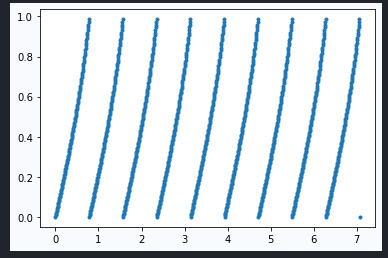
\includegraphics[width=0.7\linewidth]{img.ejem1.png}
%    \caption{}
%    \label{fig:ejemple1}
%\end{figure}



%\end{example}
Las ecuaciones impulsivas se pueden generalizar para casos donde actúen fuerzas no impulsivas $f(t,x)$ y/o donde se aplique una cantidad infinita de impulso. Un caso general se puede ver en \cite{Bainov}, el cual es

	\begin{equation*}
		\left\lbrace \begin{array}{l}
			x''=f(t,x(t)) \; \text{si }\; t\neq t_k\\
			 x'(t_k^+)-x'(t_k^-)=I_k \; \text{ donde }\; k=1,2,....,
		\end{array}\right. 
	\end{equation*}
donde, como vimos en el ejemplo, se pude pensar a los impulsos como suma, de deltas de Dirac concentradas en $t_k$ y la medida de Lebesgue $d\lambda$.\index[Simbolo]{$d\lambda$}
$$x''=f(t,x(t)) d\lambda +\sum_{k=1}^{\infty}\dfrac{I_k}{m}\;d\delta_{t_k}$$

Para resolver ecuaciones como \ref{eq:problema A}, usaremos una metodología inspirada en el libro de Pablo Amster \cite{Amster}, sobretodo en la sección 1.3. Allí utiliza el método Shooting para hallar soluciones al problemas de contorno periódico 

	\begin{equation*}
		\left\lbrace \begin{array}{l}
			u'=f(t,u(t))\\
			u(0)-u(T)=0,
		\end{array}\right. 
	\end{equation*}
donde $f$ es una función continua y Lipschitz en la segunda variable $u\in\rr^2$.  La idea que propone Pablo Amster es buscar una solución $u_\alpha$ al problema de valores iniciales 
	\begin{equation*}
	\left\lbrace \begin{array}{lcl}
		u'&=&f(t,u(t))\\
		u(0)&=&\alpha,
	\end{array}\right. 
\end{equation*}
y buscar un valor de $\alpha\in\rr^2$ tal que $u_\lambda(T)=\alpha$. No es otra cosa que un punto fijo dell operador (operador de Poíncare\index{operador de Poíncare}) $P:\rr^2\to \rr^2$, definido como $P(\alpha)=u_\alpha(T)$. Aplicando el Teorema de Brouwer \cite{Amster} al operador podemos asegurar la existencia de la solución al problema periódico. 

En el capitulo 2 haremos una breve introducción a la medida de Lebesgue-Stieltjes y sus propiedades.  En la sección 3.1 vamos a ver como transformar el problema \eqref{eq:problema A} con medidas vectoriales a uno donde intervenga una sola medida positiva, en la sección 3.2 veremos las condiciones para la existencia de soluciones al problema de valores iniciales y su continuación a intervalos máximos. En la sección 3.3 enunciaremos y demostraremos una versión del teorema de Gronwall que hemos obtenidos para medidas de Borel. A partir de este teorema demostramos la continuidad del operador de Poíncare y finalmente podremos usar el Teorema Brouwer y  hallaremos un punto fijo para el operador de Poincaré.  

\chapter{Medida de Lebesgue-Stieltjes}




En este trabajo denotaremos por $\rr$ al conjunto de todos los números reales, y por $\rr^n$ al conjunto de todas las $n$-uplas con componentes reales.  Si $x\in \rr^n$ escribimos la norma euclídea como $|x|=\sqrt{x_1^2+\cdots x_n^2}$\index[Simbolo]{$\vert x\vert$}, otra norma euclídea que usaremos sera $|x|_1=|x_1|+\cdots +|x_n|$. \index[Simbolo]{$\vert x\vert_1 $}  Usaremos el producto interno usual en $\rr^n $ definido por  $x\cdot y=x_1y_1 + \cdots+
x_ny_n$. Se pude pensar al vector $x$ como una matriz de $n\times 1$, y notaremos $x^*$ \index[Simbolo]{$x^*$}a la matriz traspuesta, $1\times n$ de $x$.

El conjunto de todas las funciones continuas, $f:[0,T]\to \rr^n$ será denotado como $C([0,T],\rr^n)$ o simplemente $C([0,T])$\index[Simbolo]{$C([0,T])$} si su codominio es $\rr$.    Escribiremos $f'(x)$ para la derivada de funciones escalares como para funciones vectoriales. 

Sea $\mathcal{X}$ un espacio topológico llamaremos $\sigma$-álgebra  de Borel\index{$\sigma$-álgebra} a la $\sigma$-álgebra generada por los conjuntos abiertos de $\mathcal{X}$, y la  denotaremos $\mathscr{B}(\mathcal{X})$. \index[Simbolo]{$\mathscr{B}(\mathcal{X})$}
En particular $\mathscr{B}(\rr)$ \index[Simbolo]{$\mathscr{B}(\rr)$}sera la $\sigma$-álgebra generada por los intervalos abiertos de $\rr$ y $\mathscr{B}([a,b])$\index[Simbolo]{$\mathscr{B}([a,b])$} la generada por los intervalos abiertos relativo de $[a,b]$. Diremos que una medida es de Borel si esta definida sobre $\sigma$-álgebra de Borel.\index{$\sigma$-álgebra!Borel}
Sea $A$ y $B$ dos conjuntos, notaremos $A\setminus B$\index[Simbolo]{$A\setminus B$} al complemento de $B$ respecto de $A$.




\section{Funciones de variación acotada}



\begin{defi}
	Dada $u:[0,T]\to \rr$, definimos la variación \index{variación!} de $u$ como \index[Simbolo]{$\V(u,[0,T])$}
	$$\V(u,[0,T])=\sup_{\substack{ t_i\in [0,T]\\
			0\leq t_1 < t_2< \dots < t_n  \leq T}}\left\lbrace \sum_{i=1}^{n}|u(t_{i+1})-u(t_i)|\right\rbrace $$
\end{defi}
\begin{defi}
	Una función $u:[0,T]\to \rr$ es de variación acotada\index{variación!acotada} en el intervalo $[0,T]$ si $\V(u,[0,T])<\infty$. \\
	El conjunto de todas las funciones de variación acotada en $[0,T]$ se denota como $BV([0,T],\rr)$.\index[Simbolo]{$BV([0,T],\rr)$} 
	Si además $u(0)=u(T)$ entonces diremos que $u\in BV_T([0,T],\rr)$. \index[Simbolo]{$BV_T([0,T],\rr)$}
\end{defi}
\begin{thm}\label{T-VB}
	 $u\in BV([0,T],\rr)$ si y sólo si $u$ se puede escribir como la diferencia de dos funciones crecientes en $[0,T]$.
\end{thm}

La demostración de este teorema o más información sobre funciones de variación acotada puede encontrarse en \cite[Teorema  2.7.2]{Carter} %(Teorema  2.7.2). 
\begin{cor}
	Si $u\in BV([0,T],\rr)$, entonces 
	\begin{itemize}
		\item para $0<t<T$ los siguientes límites existen y son finitos
		$$u(t^+)=\lim\limits_{s\to t^+}u(s) \ \ \ \ u(t^-)=\lim\limits_{s\to t^-}u(s);$$\index[Simbolo]{$u(t^+)$}
		\item $u(0^+)$ y $u(T^-)$ existen y son finitos.
	\end{itemize}
\end{cor}






\section{Medida de Lebesgue-Stieltjes}

El siguiente resultado esta demostrados en \cite[Proposición 1.2]{folland} y en \cite[Proposición 1.7]{folland}, y muestra que la $\sigma$-álgebra de Borel esta generada por intervalos de la forma $[a,b)$.

\begin{prop}\label{prop:algebra de borel}Sea $\mathcal{A}$ \index[Simbolo]{$\mathcal{A}$}la colección de todos los conjuntos que se escriben como unión finita de intervalos disjuntos de la forma $[a,b)$ con $-\infty<a<b\leq\infty$, más el conjunto $\emptyset$.
	\begin{itemize}
		\item $\mathcal{A}$ es un álgebra.\index{álgebra}
		\item La $\sigma$-álgebra generada por $\mathcal{A}$ es la $\sigma$-álgebra de Borel, ($\mathscr{B}(\rr)$).\index{$\sigma$-álgebra}\index[Simbolo]{$\mathscr{B}(\rr)$}
	\end{itemize}
\end{prop}

Sea $u:\rr \to \rr$  creciente y continua a izquierda y sea $[a_j,b_j)$ intervalos disjuntos para $j=1, \cdots ,m$. Por la \cite[Proposición 1.15]{folland},  $\mu_{0}$ definida como 

$$\mu_{0}\left( \bigcup_{j=1}^m[a_j,b_j)\right)  =\sum_{j=1}^{m}\left(u(b_j)-u(a_j)\right) $$\index[Simbolo]{$\mu_{0}$}
es una premedida \index{premedida} en $\mathcal{A}$ y a partir de una premedida podemos definir  medida exterior en $\mathscr{B}(\rr)$\index{medida! exterior} de la siguiente manera 
$$\mu^{*}(E)=\inf\left\lbrace \sum_{ j=1 }^{\infty}\mu_{0}(A_j) \mid \ A_j\in \mathcal{A}, \ \  E\subset\bigcup_{j=1}^{\infty}A_j \right\rbrace. $$\index[Simbolo]{$\mu^{*}$}
La demostración se puede ver en \cite[Proposición 1.13]{folland}.
%A partir de la medida exterior podemos definir los conjuntos $\mu$-medibles.
\begin{defi}
	Si $u:\rr \to \rr$ es creciente y continua a izquierda, llamaremos medida de Lebesgue-Stieltjes $\mu_{u}$ a la medida inducida por $\mu_{0}$. \index{medida! Lebesgue-Stieltjes}
\end{defi}

El siguiente teorema nos permite escribir a cualquier medida finita sobre la $\sigma$-álgebra de Borel, como una medida de Lebesgue-Stieltjes  . La demostración es análoga a  \cite[Teorema  1.16]{folland}.

\begin{thm}\label{medidas}
	Si $u:\rr \to\rr$ es creciente y continua a izquierda, existe una única medida de Borel $\mu_{u}$ tal que $\mu_{u}([a,b))=u(b)-u(a)$\index[Simbolo]{$\mu_u$} para todo $a$,$b$. Si $G$ es otra función creciente y continua a izquierda, entonces  $\mu_{u}=\mu_{G}$ si y sólo si $u-G$ es constante. Inversamente, si $\mu$ es una medida de Borel  en $\rr$ finita sobre cualquier conjunto acotado de Borel sea
	$$F(x)= \left\{ \begin{array}{lcc}
		\mu([0,x)) &   si  & x > 0 \\
		0 &   si  & x = 0 \\
		-\mu([0,-x)) &   si  & x < 0. 
	\end{array}
	\right. $$
	$F$ es creciente y continua izquierda, y $\mu=\mu_{F}$
\end{thm}  




%
%\begin{defi}
%Sea $u:\rr\to \rr$ una función monótona no decreciente y $[a,b)\subset\rr$ definimos la $u$-medida de $[a,b)$ como \index{medida de Lebesgue-Stieltjes} $\mu_{u}$:
%$$\mu_{u}([a,b)) =\lim\limits_{x\to b^-}f(x) - \lim\limits_{x\to a^+}f(x)=f(b^-)-f(a^+).$$
%\end{defi}

\begin{obs}
	\begin{itemize} 
		\item Si $u(x)=x$ entonces la medida $\mu_{u}$ no es otra que la medida de Lebesgue.
		\item Si $u$ es continua   en $x$, entonces usando  \cite[Teorema 3.28]{Zo} tenemos que 		
		\begin{equation*}
            \begin{split}
			\mu_{u}(\{x\})&=\mu_{u}\left( \bigcap_{n=1}^{\infty}[x,x+1/n)\right) =\lim_{n \to \infty}\mu_{u}[x,x+1/n)
			\\ &=\lim_{n \to \infty}u(x+\frac{1}{n})-u(x)=u(x)-u(x)=0
            \end{split}
		\end{equation*}
		%$$\mu_{u}(\{a\})=u(a)-u(a)=0$$		
		
		\item  Si $u$ es continua  en $b$ entonces 
		$$\mu_{u}([a,b])=\mu_{u}\left([a,b) \bigcup\{b\}\right)=\mu_{u}([a,b))=u(b)-u(a)$$		
	\end{itemize}
\end{obs}

\subsubsection{Medida de  Lebesgue-Stieltjes en un dominio acotado}
 Como $\mathscr{B}([a,b])$ \index[Simbolo]{$\mathscr{B}([a,b])$} es la $\sigma$-álgebra de Borel restringida al intervalo $[a,b]$,  por \ref{prop:algebra de borel} está generada por la familia de intervalos $\mathcal{E}=\left\lbrace [a,x) \mid x\leq b\right\rbrace $.\index[Simbolo]{$\mathcal{E}$}.
 
Sea $u:[a,b]\to\rr$ una función  monótona y continua a izquierda, podemos extender su dominio a todos los números reales, de la siguiente forma:
$$\overline{u}(t)=\left\lbrace \begin{array}{rll}
	u(a) &si & t<a\\
	u(t) & si & a\leq t < b\\
	u(b)& si & t\geq b 
\end{array}\right. $$ \index[Simbolo]{$\overline{u}$}

\begin{obs}
	\begin{itemize}
		\item $\overline{u}$ es monótona, continua a izquierda y en $b$ es continua.
		\item La medida de Lebesgue-Stieltjes generada por $\overline{u}$ cumple que 
		\begin{itemize}
			\item $\mu_{\overline{u}}(\{b\})=0,$
			\item $\mu_{\overline{u}}([a,b])=\mu_{\overline{u}}([a,b)).$
		\end{itemize}
	\end{itemize}
\end{obs}
\begin{defi}
	Sea $u:[a,b]\to\rr$ una función  monótona y continua a izquierda,  definimos la medida de Lebesgue-Stieltjes $\mu_u$ de la siguiente manera,  para $A\subset[a,b]$
	$$\mu_{u}(A)=\mu_{\overline{u}}(A)=\inf\left\lbrace \sum_{ j=1 }^n[\overline{u}(b_j)-\overline{u}(a_j)] \mid A\subset \bigcup_{j=1}^n[a_j,b_j)\right\rbrace. $$
	
	
\end{defi}

\begin{obs}
	\begin{itemize}
        \item $\mu_{u}([a,b])=\mu_{\overline{u}}([a,b])=\overline{u}(b)-\overline{u}(a)=u(b)-u(a),$
		\item Sea $[s,t)\subset[a,b]$ entonces $$\mu_{u}([s,t))=\mu_{\overline{u}}([s,t))=\overline{u}(t)-\overline{u}(s)=u(t)-u(s),$$
		
		\item Sea$[s,t)\supset[a,b]$ entonces
		$$\mu_{u}([s,t))=\mu_{\overline{u}}([s,t))=\overline{u}(t)-\overline{u}(s)=u(b)-u(a).$$
	\end{itemize}
\end{obs}








Ahora podemos definir la medida de Lebesgue-Stieltjes generada por una función de variación acotada.
\begin{thm} \label{Thm:medidas}
	Sea $u\in BV([a,b],\rr)$ y continua a izquierda, existe una medida de Borel $\mu_{u}$ tal que para todo intervalo $[a,b)$ vale que $\mu_{u}([a,b))=u(b)-u(a)$. Además para cualquier función $\mu_{u}$-integrable, $f$ y cualquier conjunto de Borel $A$ notaremos
	$$\int_{A}f(s)\;d\mu_{u}(s)=\int_{A}f(s)\;du(s).$$  \index[Simbolo]{$du$}
\end{thm}
\begin{proof}[Dem.]
Por el teorema \ref{T-VB}, si $u\in BV([a,b],\rr)$ y es continua a izquierda entonces existen $u_1$ y $u_2$ funciones monótonas y continuas a izquierda tal que $u=u_1-u_2$. Luego por el teorema \ref{medidas} las medidas generadas por $u_1$ y $u_2$ son medidas de Borel. Luego si llamamos  $\mu_u=\mu_{u_1}-\mu_{u_2}$  entonces
$$\mu_{u}([a,b))=u(b)-u(a).$$
\end{proof}


\section{Teorema de Lebesgue-Radon-Nikodyn}
Las siguientes definiciones y resultados están basados en \cite[Capitulo 3]{folland}.
%\begin{defi}
	%Sea $\mu:\mathscr{B}(I)\to \rr$ una medida finita llamaremos $\mu^+$
%\end{defi}
\begin{defi}
	Diremos que la medida $\nu$ es absolutamente continua \index{medida! absolutamente continua} respecto de la medida $\mu$, y lo notaremos $\nu\ll\mu$\index[Simbolo]{$\ll$}, si $\nu(A)=0$ cada vez que  $\mu(A)=0$.
\end{defi}
\begin{defi}
	Diremos que dos medidas $\mu$ y $\eta$ son mutuamente singulares \index{medida! mutuamente singulares}, y lo notaremos $\mu\perp \eta$,  si existen conjuntos $E,F\in\mathscr{B}([0,T])$ disjuntos tal que $E\bigcup F=[0,T]$, $\mu(E)=0$ y $\eta(F)=0$. \index[Simbolo]{$\perp$}
\end{defi}
\begin{defi}
	Diremos que una medida $\mu:\mathscr{B}(I)\to \rr$ es continua \index{medida! continua} si para todo $t\in I$ $\mu(\{t\})=0$
\end{defi}
\begin{obs}
	Si $h$ es continua entonces la medida $\mu_{h}$ es continua. Pues $\forall t\in[0,T]$
 \begin{equation*}
	\begin{split}
		\mu_{h}(\{t\})&= \mu_{h}\left( \bigcap_{n=1}^{\infty}[t,t+1/n)\right)=\lim_{n\to \infty}\mu_{h}\left( [t,t+1/n)\right)\\&=\lim_{n\to \infty}h(t+1/n)-h(t)=h(t^+)-h(t)=0.
	\end{split}
 \end{equation*}
\end{obs}

\begin{defi}
	Diremos, que un conjunto $A$ está compactamente incluido \index{compactamente incluido} en el conjunto $B$, si y sólo si $\overline{A}$ es compacto y $\overline{A}\subset B^\circ$. Lo notaremos como $A\Subset B$.
	\index[Simbolo]{$\Subset$}
 \end{defi}
\begin{thm}
    Sea $\mu$ una medida con signo, existen $\mu^-$ y $\mu^+$ medidas positivas tal que $\mu=\mu^+-\mu^-$, y además $\mu^+\perp \mu^-$.\index[Simbolo]{$\mu^+$}\index[Simbolo]{$\mu^-$}
\end{thm}
El teorema anterior se denomina \textsc{descomposición de Jordan}\index{descomposición de Jordan} ver \cite[Capitulo 3.1]{folland} , a las medidas $\mu^+$ y $\mu^-$ se llaman variación positiva\index{variación positiva} y negativa\index{variación negativa} de $\mu$ respectivamente.

\begin{defi}
    Sea $\mu$ una medida con signo, definimos la variación total de $\mu$, como 
    \begin{equation*}
        |\mu|=\mu^+ +\mu^-
    \end{equation*}\index[Simbolo]{$\vert\mu\vert$}
    
\end{defi}
\begin{obs}
 Sea $\mu$ una medida con signo, entonces valen la siguientes propiedades: \label{obs:medida}
 \begin{itemize}
     \item Para cualquier conjunto $E$ $\mu$-medible
 \begin{equation}
     |\mu|(E)=\sup\left\{\sum_{i=1}^n|\mu(E_i)| \mid \bigcup_{i=1}^nE_i=E, \; E_i \text{ disjuntos}  \right\}
 \end{equation}
 
 \item Para cualquier función $f\in L^1(\mu)$ y $E$ un conjunto $\mu$-medible
 $$\left|\int_Ef\;d\mu\right|\leq \int_E|f|\; d|\mu|$$
 \item $ \mu^{\pm}\ll |\mu|$
 \end{itemize}
\end{obs}

\begin{defi} \index[Simbolo]{$L^{p}([0,T],\mu)$}
	Sean $\mu$ una medida de Borel positiva y  $u:[0,T]\to \rr^n$ una función $\mu$-medible. Diremos que:
	\begin{enumerate}
		\item [a)] $u\in L^p([0,T],\mu)$   con $1\leq p<\infty$ si 
		\index[Simbolo]{$\lVert u\rVert_{L^p(\mu)}$} $$\left\| u\right\|_{L^p(\mu)} =\left[ \int_{[0,T)}|u(t)|^p d\mu\right] ^{1/p}<\infty$$
		En caso de que el dominio de $u$ este sobreentendido se puede denotar simplemente como $u\in L^p(\mu)$ o caso de que $\mu$ sea la medida de Lebesgue se denotara simplemente $L^p([0,T])$.
		\item [b)] Sa $\mu$ una medida de Borel, $u\in L^\infty([0,T],\mu)$ \index[Simbolo]{$L^\infty([0,T],\mu)$}si \index[Simbolo]{$\lVert u \rVert_{L^\infty(\mu)}$}
		$$\left\| u\right\|_{L^\infty(\mu)}=\inf_{M}\{|u(t)|<M, \text{para } \mu \text{- c.t.p.}\}  <\infty$$
		
	\end{enumerate}
\end{defi}
\begin{defi}
	Sea $\mu$ una medida de Borel con signo, entonces definimos $L^p(\mu)=L^p(|\mu|)$
\end{defi}




\begin{thm}[Radon-Nikodyn]\label{TL-R-N}
	Sea $\rho$ una medida finita con signo y $\mu$ una medida positiva finita en el espacio $\left( [0,T], \mathscr{B}({0,T})\right) $. Entonces existen $\lambda$ y $\nu$ medidas finitas con signo tal que 
	\begin{equation*}
		\lambda\perp\mu, \quad \nu\ll\mu  \quad \text{ y }\quad \rho=\lambda+\nu.
	\end{equation*}
Más aún, existe una función $h:[0,T]\to\rr$ $\mu$-integrable tal que para todo $A\in \mathscr{B}([0,T])$
\begin{equation*}
	\nu(A)=\int_A h(s)\;d\mu(s).
\end{equation*}
\end{thm}
La siguiente proposición es consecuencia del teorema de \ref{TL-R-N} y está demostrados en \cite[Proposición 3.9]{folland}.
\begin{prop}
    \label{ob1}
	Sea $\mu$ una medida de Borel finita, y $f\in L^1(\mu)$. Si   $$\nu(A)=\int_A f\; d\mu$$ entonces para toda función $g\in L^1(\nu)$ vale que $gf\in L^1(\mu)$ y 
	\begin{equation*}
	    \int_A g(s)\;d\nu=\int_Ag(s)f(s)\;d\mu.
	\end{equation*}

\end{prop}



\begin{lem}\label{obs3}
	Supongamos que  $\nu\ll\mu$ y sea $\mu^*$ una medida tal que $\nu(A)\leq \mu^*(A)$, entonces para toda función $\psi\in L^1(\nu)$ vale que 
	$$\int_A h(r)\psi(r)\;d\mu(r)=\int_A\psi(r)\;d\nu(r)\leq \int_A\psi(r)\;d\mu^*,$$
	donde $h$ es la derivada de $\nu$ respecto a la medida $\mu$.
\end{lem}
\begin{proof}[Dem.]
La igualdad es consecuencia del teorema \ref{TL-R-N}. Veamos la desigualdad. Vaosa a tomar el conjunto $A$ como un intervalo abierto $I$ (los cuales generan la $\sigma$-álgebra de Borel).
\begin{itemize}
	\item Si $\psi$ es una función característica, es decir $\psi(t)=X_E(t)$.
	\begin{multline*}
		\int_I \psi(r) \;d\nu(r)=\int_{I\bigcap E} \;d\nu(r)=\nu \left(I\bigcap E\right)\leq \mu^*\left(I\bigcap E\right)\\
		\leq\int_{I\bigcap E} \;d\mu^*(r)=\int_I\psi(r) \;d\mu^*(r).
	\end{multline*}
\item Si $\psi$ es una función simple, dada por $\psi(t)=\displaystyle\sum_{i=1}^{m}a_iX_{E_i}(t)$ entonces
\begin{equation*}
\begin{split}
	\int_I \psi(r)\; d\nu(r)&=\sum_{i=1}^{m}\left( a_i\int_IX_{E_i}(r) \;d\nu(r)\right) \\ &\leq
	\sum_{i=1}^{m}a_i\left( \int_IX_{E_i}(r) \;d\mu^*(r)\right) =\int_I \psi(r)\; d\mu^*(r).
 \end{split}
\end{equation*}
\item Si $\psi$ es una función integrable positiva, entonces existe una sucesión de funciones simples $f_1(t)\leq f_2(t)\leq\cdots$ tal que $\lim\limits_{k\to\infty}f_k(t)=\psi(t)$. Luego, usando Beppo-Levi,
\begin{equation*}
\begin{split}
	\int_I\psi(r)\;d\nu(r)&=\lim\limits_{k\to\infty}\int_I f_k(r)\;d\nu(r)\\
	&\leq \lim\limits_{k\to\infty}\int_I f_k(r)\;d\mu^*(r)=\int_I\psi(r)\;d\mu^*(r).
 \end{split}
\end{equation*}
	\item Si $\psi$ es cualquier función integrable, entonces se puede descomponer como diferencia de dos funciones positivas, es decir $\psi=\psi^+-\psi^-$  y por lo anterior satisface  que 
$$\int_I\psi(r)\;d\nu(r)\leq \int_I\psi(r)\;d\mu^*.$$	
\end{itemize}
Luego, si se verifica para cualquier intervalo $I$ entonces como generan la $\sigma$-álgebra de Borel, se satisface para cualquier conjunto $A$ de Borel.
\end{proof}








\begin{defi}
	Sea $\mu$ una medida, llamaremos $D_{\mu}$ o simplemente $D$, al conjunto de los puntos de discontinuidad \index{punto de discontinidad} de $\mu$. Es decir, 
	$$D=\{t \in [0,T]  \mid  \mu(\{t\})\neq 0\}.$$\index[Simbolo]{$D$}
\end{defi}

\begin{lem}\label{D numerable}
	Si $\mu:\mathscr{B}([0,T])\to \rr$ es una medida finita y positiva, entonces el conjunto $D$ es numerable.
\end{lem}
\begin{proof}[Dem.]
	Para $n\in\nn$ definimos el conjunto $D_n=\{\tau|\mu(\{\tau\})>1/n\}$, entonces $D=\bigcup_{n=1}^\infty D_n$. El conjunto $D_n$ es finito, porque de lo contrario va a existir una sucesión de elementos $\{a_k\}_{k=1}^\infty\subset D_n$ tal que 
	\begin{equation*}
		\mu([0,T])\geq\mu(D_n)\geq\sum_{k=1}^{\infty}\mu(\{a_k\})>\sum_{k=1}^{\infty}\dfrac{1}{n}=\infty,
	\end{equation*}
	lo cual es un absurdo pues $\mu$ es una medida finita. Por lo tanto, $D_n$ es finito y $D$ es la unión numerable de conjuntos finitos. 
\end{proof}


\chapter{Soluciones periódicas a MDE}




\section{Medidas vectoriales}

En el  ejemplo \ref{ejemplo1} del capitulo 1, al  problema impulsivo \eqref{eq:imp} lo escribimos como una MDE de la siguiente manera
\begin{equation*}
	x''(t)=\sum_{k=1}^{r}\dfrac{I_k}{m}\delta_{t_k}.
\end{equation*}
Si  realizamos la sustitución $v=x'$ tendremos el sistema
\begin{equation*}
	\left( x',v'\right) =\left( v ,\dfrac{1}{m}\right) \cdot \left( d\lambda, \displaystyle\sum_{k=1}^{r}I_k\delta_{t_k}\right) , 
\end{equation*}
el término de la derecha del producto escalar es un vector de medidas o una medida vectorial.  En \cite{distel} se define medida vectorial para espacios de Banach $X$. Sin embargo en nuestro caso, es $X$  un espacio euclídeo  $m$-dimensional, y llamaremos medida vectorial a $\nu=(\nu_1,\nu_2,...,\nu_m)$ donde cada $\nu_i$ es una medida de Borel con signo.  La variación total de una medida vectorial $\nu$ se define para un conjunto de Borel $E$, (ver definición 4 de \cite{distel}, tomando $\rr^m$ con la norma de $l^1$) como 
$$||\nu||(E)=sup\left\{ \sum_{j=1}^r |\nu(E_j)| _1 \mid \bigcup_{j=1}^rE_j=E\right\}$$
donde $|\nu(E_j)|_1=\displaystyle\sum_{i=1}^m|\nu_i(E_j)|$.
\begin{lem}
    Sea $\nu=(\nu_1,\nu_2,...,\nu_m)$ una medida vectorial y $E$ un conjunto de Borel, entonces
    \begin{equation}
        ||\nu||(E)=\sum_{i=1}^{m}|\nu_i|(E). 
\end{equation}\index[Simbolo]{$\Vert \nu \Vert$}
\end{lem}
\begin{proof}[Dem.]
    Por  \eqref{obs:medida} y como $\displaystyle|\nu(E)|_1= \sum_{i=1}^{m}|\nu_i(E)|$
    \begin{equation*}
    \begin{split}
       \sum_{i=1}^{m} |\nu_i|(E)&=\sum_{i=1}^{m} \left[sup\left\{ \sum_{j=1}^r |\nu_i(E_j)| \mid \bigcup_{j=1}^rE_j=E\right\} \right]\\
       \sum_{i=1}^{m} |\nu_i|(E) &\geq sup\left\{ \sum_{i=1}^{m} \sum_{j=1}^r |\nu_i(E_j)| \mid \bigcup_{j=1}^rE_j=E \right\}\\
       \sum_{i=1}^{m} |\nu_i|(E) &\geq sup\left\{  \sum_{j=1}^r \sum_{i=1}^{m} |\nu_i(E_j)| \mid \bigcup_{j=1}^rE_j=E \right\}\\
       \sum_{i=1}^{m} |\nu_i|(E) &\geq ||\nu||(E)
    \end{split}
    \end{equation*}
Sea $E_i^{+}$ y $E_i^-$  la descomposición de Hahn del conjunto $E$ respecto de la medida $\nu_i$ (ver \cite{folland}), entonces $|\nu_i|(E)=\nu_i(E_i^+)+\nu_i^-(E_i^-)$.    Defino el conjunto finito de subindices  $I=\{\alpha\in\rr^m,  \; | \: \alpha_i\in\{+,-\} \}$, luego para cada $\alpha\in I$ defino el conjunto $F_\alpha=\displaystyle\bigcap_{i=1}^mE_i^{\alpha_i}$. Si $\alpha,\beta\in I$ y $\alpha\neq\beta$ entonces existe $i$ tal que  $\alpha_i\neq\beta_i$,  y por lo tanto $E_i^{\alpha_i}\cap E_i^{\beta_i}=\emptyset$ y $E_i^{\alpha_i}\cup E_i^{\beta_i}=E$. De este hecho  podemos afirmar que para  $\alpha\neq\beta$ se cumple que
  \begin{equation*}
  	\begin{split}
  		F_\alpha\cap F_\beta&=\bigcap_{i=1}^mE_i^{\alpha_i}\cap \bigcap_{i=1}^mE_i^{\beta_i}=\bigcap_{i=1}^mE_i^{\alpha_i}\cap E_i^{\beta_i}=\emptyset.
  	\end{split}
  \end{equation*}
  Es decir la familia $\left\lbrace F_\alpha\right\rbrace _{\alpha\in I}$ es una familia de conjuntos mutuamente disjuntos.  Además
  \begin{equation*}
      \begin{split}
        \bigcup_{\substack{\alpha\\ \alpha_i=+}}F_\alpha&=\bigcup_{\substack{\alpha\in I\\ \alpha_i=+}}\left( E_1^{\alpha_1}\cap..\cap  E_i^+\cap...\cap E_m^{\alpha_m} \right)\\
        &=E_i^+\bigcap \left(\bigcup_{j=1}^m E_j^+\cap E_j^- \right)=E_i^+\cap E=E_j^+
      \end{split}
  \end{equation*}
  
  
  
  
  Luego para $i=1,...,m$ 
  \begin{equation*}
  	|\nu_i|(E)=\nu_i \left( \bigcup_{\substack{\alpha\\ \alpha_i=+}}F_\alpha\right) + \nu_i \left( \bigcup_{\substack{\alpha\\ \alpha_i=-}}F_\alpha\right)= \sum_{\substack{\alpha\\ \alpha_i=+}}\nu_i(F_\alpha)+\sum_{\substack{\alpha\\ \alpha_i=-}}\nu_i(F_\alpha)
  \end{equation*}
  Como $F_{\alpha}$ con $\alpha_i=+$ está incluido en $E_i^+$ entonces $\nu_i(F_\alpha)>0$ si $\alpha_i=+$, y por lo mismo $\nu_i(F_\alpha)>0$ si $\alpha_i=-$. Por lo tanto
  \begin{equation*}
  	|\nu_i|(E)= \sum_{\substack{\alpha\\ \alpha_i=+}}|\nu_i(F_\alpha)|+\sum_{\substack{\alpha\\ \alpha_i=-}}|\nu_i(F_\alpha)|=\sum_{\substack{\alpha}}|\nu_i(F_\alpha)|,
  \end{equation*}
  entonces
   \begin{equation*}
  	\sum_{i=1}^{m}|\nu_i|(E)=\sum_{i=1}^{m}\left( \sum_{\substack{\alpha}}|\nu_i(F_\alpha)|\right) = \sum_{\substack{\alpha}}\sum_{i=1}^{m}|\nu_i(F_\alpha)|.
  \end{equation*}
  Por lo tanto
  \begin{equation*}
  	\sum_{i=1}^{m}|\nu_i|(E)= \sum_{\substack{\alpha}}|\nu(F_\alpha)|\leq ||\nu||(E).
  \end{equation*}
 
\end{proof}
\begin{obs}

Por \eqref{obs:medida} $\nu_i\ll |\nu_i|$ y por el lema anterior cada $|\nu_i|$ es absolutamente continua respecto a la medida $||\nu||$, entonces para toda $i=1,..., m$ vale que $\nu_i\ll ||\nu||$.\label{obs:R-D}
	Por el teorema Radon-Nikodyn \eqref{TL-R-N}, para cada $i=1,..., m$ existe $h_i\in L^1(||\nu||) $ tal que para todo conjunto de Borel $A$
	$$\nu_i(A)=\int_A h_i(s)\;d||\nu||(s).$$
 \end{obs}
 \begin{prop}\label{prop:medida vectorial}
    Para toda medida vectorial $\nu$, existe $H\in L^1(\rr^m,||\nu||)$, tal que para todo conjunto de Borel $A$
    \begin{equation*}
		\nu(A)=\int_A H(s)\;d||\nu||.
	\end{equation*}
 \end{prop}
\begin{proof}[Dem.]
    Basta con aplicar la observación \eqref{obs:R-D}
\end{proof}     

	
\subsubsection{Ecuaciones con medidas vectoriales}

Sea $F:[0,T]\times\rr^n\to \rr^{n\times m}$ con $F(t,x)$  continua y  localmente Lipschitz con respecto a $x$, y $\nu$ una medida vectorial con valores en   $\rr^m$ \index{medida! vectorial}.
Vamos a considerar la ecuación 

\begin{equation}\label{eq:8}
d\varphi(t)=F(t,\varphi(t))d\nu . 
\end{equation}
\begin{defi}
	Una solución de \eqref{eq:8} es una función $\varphi\in BV([0,T],\rr^n)$ y continua a izquierda tal que  
\begin{equation}\label{eq:9}
    \varphi(t)-\varphi(0)=\int_{[0,t)}d\varphi=\int_{[0,t)}F(s,\varphi(s))\; d\nu.
\end{equation}
\end{defi}

\begin{thm}\label{thm:m_equivalente}
Una solución de \eqref{eq:8} es también solución de    
\begin{equation}\label{eq:10}
	d\varphi=f(t,\varphi(t))d\mu
\end{equation} 
donde $f=F[H]^*:[0,T]\times\rr^n\to \rr^n$ y  $\mu$ es una medida de Borel positiva. 
\end{thm}
\begin{proof}[Dem.]
    De la proposición \eqref{prop:medida vectorial} existe $H:\rr^m\to\rr^n$ en  $L^1(||\nu||)$ tal que  podemos escribir la definición \eqref{eq:9} como 
    \begin{equation*}
        \begin{split}
           \varphi(t)-\varphi(0)=\int_{[0,t)}F(s,\varphi(s))\; d\nu=\int_{[0,t)}F(s,\varphi(s))[H(s)]^\tau\; d||\nu||
        \end{split}
    \end{equation*}



De esta manera, podemos decir que la solución de \ref{eq:8}, es también solución de un problema donde la medida que intervine no es vectorial. En efecto si llamamos $f(t,x)=F(t,x)[H(t)]^\tau$ y $\mu=||\nu||$

\begin{equation*}
	d\varphi=f(t,\varphi(t))d\mu
\end{equation*} 
donde $f:[0,T]\times\rr^n\to \rr^n$ y  $\mu$ es una medida de Borel positiva.
\end{proof}


 \begin{example}
 	Sea $\varphi:[0,T]\to\rr$ solución de  
 	\begin{equation}
 		d\varphi=F(t,\varphi)+\sum_{k=1}^rg_k(t)\;d\delta_{t_k},\label{eq:ejemplo 1}
 	\end{equation}
  donde $g_i:[0,T]\to \rr$ son funciones continuas, $F$ es suficientemente buena, cuando $F$ no este acompañada de ninguna media  vamos a convenir que se trata de la medida de Lebesgue $d\lambda$. A la expresión anterior la podemos escribir de manera vectorial como 
 	\begin{equation*}
	d\varphi=\left( F(t,\varphi(t)),g_1(t),...,g_r(t)\right)  \left( d\lambda, d\delta_{t_1},...,d\delta_{t_r}\right)^\tau. 
\end{equation*} 
 Si llamamos $\nu=(\lambda,\delta_{t_1},...,\delta_{t_r})$ y aplicamos el teorema \eqref{thm:m_equivalente} tenemos que  $||\nu||=\displaystyle\lambda+\sum_{k=1}^r\delta_{t_k}$, y como
$$\delta_{t_k}(A)=\int_A  \chi_{\{t_k\}}\; d||\nu||,$$
%$$\delta_{t_2}(A)=\int_A  \chi_{\{t_2\}}\; d||\nu||,$$
$$\lambda(A)=\int_A \chi_{A-\{t_1,..t_r\}}\; d||\nu||,$$
entonces llamando $H(t)=(1,\chi_{\{t_1\}},..,\chi_{\{t_r\}})$  la solución de \eqref{eq:ejemplo 1} es también solución de la ecuación 

 	\begin{equation*}
	d\varphi=\left(F(t,x),g_1(t),...,g_r(t)\right)H(t)^\tau \; d||\nu||
\end{equation*} 
 tomando $f(t,x)=(F(t,x),g_1(t),...,g_r(t))H(t)^\tau$ y $||\nu||=\mu$ entonces  $\varphi$ es solución de


 	\begin{equation*}
	d\varphi=f(t,\varphi)\; d\mu,
\end{equation*} 
 \end{example}
 %%%%%%%%%%%%%%%%%%%%%%%%%%%%%%%%%%%%%%%%%%%%%%%%%%%
 %TEOREMA DE EXISTENCIA Y UNICIDAD SIN MEDIDA
 %%%%%%%%%%%%%%%%%%%
 
% \begin{thm}[Existencia y Unicidad] \label{EyU}
% 	Sea $a\in\rr$, $b\in\rr^n$ y $f:\Omega=[t_0-a,t_0+a]\times[x_0-b,x_0+b]\to\rr^n$ continua y localmente Lipschitz en la variable $x$. El problema 
% 	$$ \left\{ \begin{array}{lc}
% 	x'(t)=f(t,x(x)) &     \\
% 	x(0)=x_0 &
% 	\end{array}
% 	\right. $$
% 	admite una única solución $x:(t_0-\delta,t_0+\delta)\to \rr^n$ para $\delta=\min\{a,b/M\}$ donde $M=\displaystyle\sup_{\|x\|<1}\{|f(x)|\}$
% 	\end{thm}
% 
% 
% 
% 	\begin{lem}[Lema de Granwal] \label{L-Granwall}
% 		Sea $u,v:[t_0,t_1]\to [0,\infty)$ continuas tal que 
% 		$$u(t)\leq\alpha +\int_{t_0}^{t_1}u(s)v(s)ds \ \ \forall t \text{ y algun } \alpha>0$$
% 		Entonces $u(t)\leq \alpha e^{\int_{t_0}^{t_1}v(s)ds}$
% 	\end{lem}
% 
% 
% 
% Bajo las hipótesis del Teorema de Existencia y Unicidad \ref{EyU} si tomamos $(\tilde{t_0},\tilde{x_0})\in[t_0-\frac{\delta}{3},t_0+\frac{\delta}{3}]\times[x_0-\frac{b}{3}, x_0+\frac{b}{3}]$ y tomamos como $\Omega=[t_0-\frac{\delta}{2},t_0+\frac{\delta}{2}]\times[x_0-\frac{b}{2},x_0+\frac{b}{2}]$ entonces $(\tilde{t_0},\tilde{x_0})\in\Omega$ y el PVI
% 
% $$ \left\{ \begin{array}{lc}
% x'(t)=f(t,x(x)) &     \\
% x(\tilde{t_0})=\tilde{x}+_0 &
% \end{array}
% \right. $$
%Tiene una única solución $\tilde{x}(t):(\tilde{t}_0-\tilde{\delta},\tilde{t}_0+\tilde{\delta})\to \rr^n$, donde $\tilde{\delta}=min\{\frac{\delta}{2},\frac{b}{2M}\}$, pero como ya teníamos que $\delta\leq\frac{b}{M}$ entonces $\frac{\delta}{2}\leq\frac{b}{2M}$, es decir $\frac{\delta}{2}=\tilde{\delta}$. Así $\tilde{x}(t):(\tilde{t}_0-\frac{\delta}{2},\tilde{t}_0+\frac{\delta}{2})\to \rr^n$
%
%Luego $\forall t\in [\tilde{t}_0-\frac{\delta}{6},\tilde{t}_0+\frac{\delta}{6}]$ tanto $x$ como $\tilde{x}$ estan bien definidas y son continuas. Por lo tanto para 
%
%$$x'(t)-\tilde{x}'(t)=f(t,x(t))-f(t,\tilde{x}(t))$$
%
%$$x(t)-\tilde{x}(t)=x(t_0)-\tilde{x}(t_0)+\int_{t_0}^{t}f(s,x(s))-f(s,\tilde{x}(s))ds$$
%
%Luego si suponemos que $t_0<\tilde{t_0}<t<\tilde{t_0}+\frac{\delta}{6}$
%\begin{multline*}
%|x(t)-\tilde{x}(t)|\leq |x(t_0)-\tilde{x}(t_0)|+\int_{t_0}^{t}|f(s,x(s))-f(s,\tilde{x}(s))|ds\leq|x(t_0)-\tilde{x}(t_0)|+L\int_{t_0}^{t}|x(s)-\tilde{x}(s)|ds\\
%|x(t)-\tilde{x}(t)|\leq|x(t_0)-\tilde{x}(t_0)|+L\int_{t_0}^{t}|x(s)-\tilde{x}(s)|ds
%\end{multline*}
% Si llamo $\alpha=|x(t_0)-\tilde{x}(t_0)|$, $v(t)=L$, $u(t)=|x(t)-\tilde{x}(t)|$ y $[t_0,t_1]=[t_0,\tilde{t_0}+\frac{\delta}{6}] $ podemos aplicar el Lema de Granwal \ref{L-Granwall} tenemos que 
% $$|x(t)-\tilde{x}(t)|\leq |x(t_0)-\tilde{x}(t_0)|e^{L(t-t_0)}$$
%Si definimos $\phi(t,t_0,x_0):=x(t)$ entonces tenemos que 
% $$|\phi(t,t_0,x_0)-\phi(t,\tilde{t_0},\tilde{x_0})|=|x(t)-\tilde{x}(t)|\leq |x(t_0)-\tilde{x}(t_0)|e^{L(t-t_0)}\to 0$$
%cuando $(\tilde{t_0},\tilde{x_0})\to (t_0,x_0)$.
%Es decir $\phi$ es continua con respecto a $(t_0,x_0)$.
%Luego para el problema \ref{P-Primer-Orgen}, si tomamos $t_0=0$ y $v_0=(\lambda_1,\lambda_2)$ entonces $\phi(1,t_0,v_0)=v_{\lambda}(1)$, resulta continua para cualquier valor de $\lambda\in\rr^{2n}$. 
%
%


%
% \subsection{Operador de Poincaré}
% Para el problema periódico
% $$ \left\{ \begin{array}{lc}
% 	u'(t)=f(t,u(x)) &     \\
% 	u(0)=u(1) 
% \end{array}
% \right. $$ 
% donde $f$ es continua y localmente Lipschitz en u.
%Sea $u_{\lambda}$ la solución al problema de valores iniciales
%  $$ \left\{ \begin{array}{lc}
%  	u'(t)=f(t,u(x)) &     \\
%  	u(0)=\lambda 
%  \end{array}
%  \right. $$
% para algún $\lambda\in \rr^n$
% Definimos el operador de Poincaré $P(\lambda)=u_{\lambda}(1)$ siempre y cuando $u_{\lambda}$ este definida en $[0,1]$.
% Ademas necesitamos que $P(\lambda)$ sea continuo y que $P(\hat{B(0,1)})\subset \hat{B(0,1)}$ entonces por el Teorema de Brouwer, el operador de Poincaré tiene un punto fijo, es decir $P(\lambda)=\lambda=u_{\lambda}(1)$. 
% 
% \begin{thm}[Teorema de Brouwer]
%Sea $B$ la bola unitaria de $\rr^n$ y sea $f : B \to B$ continua. Entonces existe $x \in B$ tal que $f (x) = x$. 	
% \end{thm}
% 
% Si $f:[0,1]\times\rr^n\to\rr^n$ es continua y localmente Lipschitz en $u$, tal que $f(t,u)\cdot u <0$ para $|u|=R$, entonces podemos asegurar que el operador de Poincaré es continuo y ademas se puede extender hasta el intervalo $[0,1]$. Así podemos aplicar el Teorema de Brouwer y asegurar que el problema periódico tiene al menos una solución.
% 
 
% 
%  \subsection{Problema de Segundo Orden}
% Sea $f:[0,1]\times\rr^n\to\rr^n$ una función $C^2(\rr)$.
% Para el problema 
% $$ \left\{ \begin{array}{lc}
% 	u''(t)=f(t,u(x)) &     \\
% 	u'(0)=u'(1) &\\
% 	u(0)=u(1) 
% \end{array}
% \right. $$
% 
% Supongamos ademas que vale la condición de \textbf{Hartman}, existe $R>0$ tal que 
% $$f(t,-R)<0<f(t,R) \ \ \text{para todo } t\in[0,T]$$
% 
% Podemos definir (¿?) una función $\tilde{f}(t,u)$, $C^2(\rr)$ tal que $\tilde{f}\equiv f$ en el rectángulo $[0,1]\times[-R,R]$ y 
% $f(t,-u)<0<f(t,u) \ \ \forall|u|\geq R\text{ y } \forall t\in[0,T]$. Entonces si tengo una solución del problema modificado
%  $$ \left\{ \begin{array}{lc}
% 	u''(t)=\tilde{f}(t,u(x)) &     \\
% 	u'(0)=u'(1) &\\
% 	u(0)=u(1) 
% \end{array}
% \right. $$
% también lo será para el problema original.
 
 
 
 
 
 
 
 
 
 
 
 
 
 
 
 
 
 
 \section{Existencia de Soluciones a MDE}
 \subsection{Soluciones locales}
 A continuación definiremos el problema de valores iniciales con medida, cuando una función $\varphi$ es solución del dicho problema y cual es el dominio máximo de esa solución.  Los resultados fueron probados por \cite{P.Mazzone}.
 Vamos a considerar el problema de valores iniciales con medida (MDE)\index{MDE}
 \begin{equation}\label{Problema P}
 	\left\lbrace \begin{array}{l}
 		d(\varphi)=f(t,\varphi(t))d\mu\\
 		\varphi(0)=x_0,
 	\end{array}\right. \tag{${P}$}
 \end{equation}
 donde $f:\Omega\subset[0,T]\times\rr^n\to\rr^{n}$, $\mu$ es una medida de Borel y $d\varphi$ es la medida de Lebesgue-Stieltjes generada por $\varphi$.

\begin{defi}
    Sea $t_0\in [0,T)$, $h>0$,  $x_0\in \rr^n$ y $r>0$, diremos que $f:\Omega=[t_0,t_0+h]\times\rr^n\to\rr^{n}$ es localmente Lipschitz \index{localmente lipschits} si  $\exists L>0$  tal que
	\begin{equation}\label{f lipschitz}
	\left\| f(t,x)-f(t,y)\right\|\leq L\left\| x-y\right\|
\end{equation}
	para todo $(t,x,y)\in I\times \overline{B(x_0,r)}\times \overline{B(x_0,r)}$.
\end{defi}

 
 \begin{defi}[\textbf{Solución del problema (P)}]
 Para el intervalo $I=[t_0,t_0+h)\subset \rr$, $\mu:I\to \rr^m$ sea una medida vectorial de Borel, $x_0\in \rr^n$  y $\Omega\subset I\times\rr^n$ un entorno abierto de $(t_0,x_0)$. Supongamos  que $f:\Omega\to \rr^{n\times m}$ cumple con
 	\begin{enumerate}[label=\upshape(\Roman*),ref=(\Roman*)]
 		\item\label{th:c1} Para cada $x\in\rr^n$, $f(t,x)$ es $\mu$-medible respecto a la variable $t$. 
 		\item\label{th:c2} Para cada $t$, $f(t,x)$ es continua respecto la variable $x$.
 		\item\label{th:c3} Existe $\alpha:\rr^n\to[0,\infty)$ continua y $\beta\in L^1(\rr,|\mu|)$ no negativa tal que 
 		$$\left\| f(t,x)\right\|\leq \beta(t)\alpha(x) .$$
 	\end{enumerate}
 	 Diremos que el par $(\varphi,I)$ es solución de \ref{Problema P} con $\varphi(t_0)=x_0$, si para todo $t\in I$, $(t,\varphi(t))\in \Omega$,  $\varphi\in BV(I,\rr^n)$   es continua a izquierda en $I$ y para todo conjunto de Borel $A$ vale que 
 	$$\mu_{\varphi}(A)=\int_{A}f(t,\varphi(t))\; d\mu.$$ 
 \end{defi}
















\begin{thm}[Picard–Lindelöf] 
	\label{P-L}
	Supongamos que $f$ está acotada (es decir $\|f\|_{\infty}\leq M$), satisface con las condiciones \ref{th:c1} y \ref{th:c2} y \ref{f lipschitz}. Asumimos que $\mu$ es una medida de Borel definida en $I$ y existe $\delta_1>0$ tal que $|\mu|([t_0,t_0+\delta_1))\leq r/M$. Si $\delta=min\{\delta_1, h\}$, el problema \eqref{Problema P} tiene una única solución en el intervalo $[t_0, t_0+\delta)$.
	
\end{thm}
 
 La demostración del teorema está en \cite[Teorema 4.1]{P.Mazzone}
 
 \subsection{Extensión de las soluciones}
 \begin{defi}[\textbf{Solución Máxima}] \index{solución máxima}
 	Sea $\Omega\subset\rr\times\rr^n$ un conjunto abierto, $f:\Omega\to\rr^n$, $(t_0,x_0)\in\Omega$ y $\mu$ una medida de Borel finita. Si $\varphi$ es solución del problema \eqref{Problema P} en el intervalo $I=[t_0,t_0+\delta)$, diremos que $(\varphi,I)$ es la solución máxima si no hay otra solución $(\psi,J)$ tal que $I\subset J$ y para todo $t\in I$ $\varphi(t)=\psi(t)$.
 \end{defi}

 \begin{defi} 
 	Sean $\mu$ una medida de Borel finita y  $f:[0,T]\times\rr^n\to\rr^n$. Diremos que $f$ cumple con la \textbf{condiciones de teletransportación}\index{condiciones de teletransportación} en  $\overline{B(0,R)}$, si  para todo $t\in[0,T]$ tal que $\mu(\{t\})\neq0$ y $x\in\overline{ B(0,R)}$ vale que 
 	\begin{equation*}
 		x+f(t, x)\mu(\{t\}) \in \overline{B(0,R)} \label{fun-tele}
 	\end{equation*}
 	donde $B(0,R)$ denota la bola abierta de $\rr^n$ de radio $R$ y centrada en el origen.\index[Simbolo]{$B(0,R)$}
 \end{defi}

\begin{thm}	\label{th:extensión}
	Sean $\mu$ una medida de Borel finita y $f$ localmente Lipschitz respecto a la variable vectorial y $\varphi$ la solución máxima de \eqref{Problema P} en $I=[t_0,t_1)$. Entonces una y sólo una de las afirmaciones es verdadera: 
	\begin{enumerate}[label=\upshape(\Roman*)]
		\item  Para todo $K\Subset\Omega$ existe $t_2\in I$ tal que $(t,\varphi(t))\notin K$ para todo $t\in(t_2,t_1)$.
		\item Existe el límite $x_1=\lim\limits_{t\to t_1^-}\varphi(t)$, tal que  $(t_1,x_1)\in\Omega$ y 
		$$\left( t_1 ,\varphi(t_1)+f(t_1,\varphi(t_1))\mu(\{t_1\})\right) \notin \Omega.$$
	
	\end{enumerate}
\end{thm}
La demostración de este resultado se puede ver en \cite[Teorema 5.5]{P.Mazzone}.

















\subsection{Teorema de Cambio de Variables}\index{Teorema de Cambio de Variables}
Vamos a demostrar una generalización del teorema de cambio de variable \cite[Teorema 6.1]{P.Mazzone}, para el caso donde $|F''|<M$, el cual usaremos para demostrar una desigualdad del tipo Gronwall.  
Empecemos enunciando el siguiente lema de cubrimiento demostrados en \cite[Corolario I, p 35]{Evanz}.



\begin{lem}[Lema de cubrimiento]
	\label{Lema de  cubrimiento}
	Sea $\mu$ una medida de Borel en $\rr^n$, y $\mathcal{F} $ cualquier colección de bolas cerradas. Sea $A$ el conjunto de los centros de las bolas en $\mathcal{F} $. Supongamos que $\mu(A)<\infty$ y $\inf\{r\mid B(a,r)\in \mathcal{F} \}=0$ para cada $a\in A$.  Entonces, para todo conjunto abierto $U\subset\rr^n$ existe una sucesión numerable $\mathcal{G} $ de bolas de $\mathcal{F} $ tal que 
	\begin{equation*}
		\bigcup_{B\in \mathcal{G} }B\subset U \quad \text{y}\quad \mu\left( (A\cap U)\setminus\bigcup_{B\in \mathcal{G} }B\right)=0. 
	\end{equation*}
	
	
\end{lem}





 \begin{thm}\label{TCV}
	Asumamos $J\subset\rr$ un intervalo abierto. Sea $F:J\to \rr$ una función diferenciable tal que $F'$ es acotada y absolutamente continua. Además,  supongamos que existe $M>0$ tal que $F''>-M$. Entonces, para toda función $g:I\to J$ creciente y  continua a izquierda,  donde $I$ es un intervalo abierto, y para todo $A\in \mathcal{B}(I)$ vale que
	$$\int_{A}F'(g(s)) \; dg\leq \mu_{F\circ g}(A)+\dfrac{M}{2}\sum_{t\in D\cap A}\mu_{g}(\{\tau\})^2,$$
donde $D=\{\tau\in I \mid \mu_{g}(\{\tau\})>0\}$.\label{Teorema medidas}
\end{thm}
Antes de comenzar con la demostración vamos a ver los siguientes lemas que nos ayudara a la desmostración.
\begin{lem}
Sea $F$ bajo las hipotesis del Teorema, para cualquier función $g:I\to J$ creciente y continua a izquierda vale que para $[a,b)\subset I$ \begin{equation}
    |\mu_{F\circ g}([a,b))|\leq R\mu_{g}([a,b)).
\end{equation}
En particular vale que $\mu_{F\circ g}\ll \mu_g$.\label{lem: abs cont}
\end{lem}
\begin{proof}[Dem.]

Para $[a,b)\subset I$, llamamos $x=g(a)$ e $y=g(b)$, como $g$ es creciente entonces $x<y$, y como $F'$ continua podemos aplicar el  teorema del valor medio del cálculo diferencial. Existe en $c\in (x,y)$ tal que 

	$$ \dfrac{|F(y)-F(x)|}{y-x} =  |F'(c)| \leq \sup_{t\in J}\left|F'(t) \right|, $$
	y como $|F'|<R$ para $R>0$, entonces
	\begin{equation} \label{eq:f'}
		 |F(y)-F(x)| \leq R (y-x).
	\end{equation}
Por lo tanto para todo intervalo $[a,b)\in I$
	\begin{equation*}
		|\mu_{F\circ g}\left( [a,b)\right)|\leq R\mu_{g}\left( [a,b)\right).
		\label{eq:medidas}
	\end{equation*}
 Sea $(a,b)\in \mathcal{B}(I)$ 
\begin{multline}\label{eq:324}
    |\mu_{F\circ g}((a,b))|=\left|\mu_{F\circ g}\left(\bigcup_{n=1}^{\infty}\left[a+\frac{1}{n},b\right)\right)\right|=\lim_{n\to \infty}\left|\mu_{F\circ g}\left(\left[a+\frac{1}{n},b\right)\right)\right|\\
    \leq R\lim_{n\to \infty}\mu_{g}\left(\left[a+\frac{1}{n},b\right)\right)=R\mu_g((a,b)).
\end{multline}
Sea $A\in \mathcal{B}(I)$, $\forall \epsilon>0$ existe $(a_i,b_i)$ una sucesión de intervalos disjuntos tal que $A\subset \displaystyle\bigcup_{i=1}^{\infty}(a_i,b_i)$ y  por  \cite[Lema 1.7]{folland} 
$$\sum_{i=1}^{\infty}\mu_{ g}(a_i,b_i)\leq \mu_g(A)+\epsilon$$
luego por \ref{eq:324}
\begin{equation}
    \mu_{F\circ g}(A)\leq \sum_{i=1}^{\infty}\mu_{F\circ g}(a_i,b_i)\leq R\sum_{i=1}^{\infty}\mu_{ g}(a_i,b_i)\leq \mu_g(A)+\epsilon.\label{eq:<}
\end{equation}
Por otro lado existe una secesión de intervalos disjuntos $(a_j,b_j)$ tal que 
$$\sum_{j=1}^{\infty}\mu_{F\circ g}(a_j,b_j)\leq \mu_{F\circ g}(A)+\epsilon,$$
usando nuevamente \ref{eq:324} tengo que 
\begin{equation*}
-R\sum_{j=1}^{\infty}\mu_{ g}(a_j,b_j)\leq \sum_{j=1}^{\infty}\mu_{F\circ g}(a_j,b_j)\leq \mu_{F\circ g}(A)+\epsilon.
\end{equation*}
Tomando supremo sobre los intervalos $(a_j,b_j)$ cuya unión numerable contienen al conjunto $A$
\begin{multline}
    -R\mu_g(A)=R\sup\left\{ -\sum_{j=1}^{\infty}\mu_{ g}(a_j,b_j)  \mid a\subset \bigcup_{j=1}^{\infty}(a_j,b_j) \right\}\\
    \leq \mu_{F\circ g}(A)+\epsilon.\label{eq:>}
\end{multline}
Luego de \ref{eq:<} y \ref{eq:>} tenemos que $\forall \epsilon>0$
\begin{equation}
    -\mu_g(A)-\epsilon\leq \mu_{F\circ g}(A)\leq  \mu_g(A)+\epsilon.
\end{equation}
por lo ranto para todo conjunto $A\in \mathcal{B}(I)$ vale que 
$$ |\mu_{F\circ g}(A)|\leq R\mu_g(A).$$
De lo anterior podemos deducir que $\forall \epsilon>0$ existe $\delta=\epsilon/R$ tal que si $\mu_g(A)\leq \delta$ entonces $|\mu_{F\circ g}(A)|\leq \epsilon$, y por el   \cite[Teorema 3.5]{folland} es necesario y suficiente para que $\mu_{F\circ g} \ll \mu_g$.



\end{proof}

\begin{lem}\label{lem: g cont}
    Asumamos $J\subset \rr$ un intervalo abierto. Sea $F:J\to \rr$ con las hipotesis del Teorema \eqref{TCV}. Entonces, para cualquier función continua y creciente $g:I\to J$, donde I es un intervalo abierto, y para todo $A\in \mathcal{B}(I)$ vale que
    \begin{equation}
        \int_{A}F'(g(s)) \;dg=\mu_{F\circ g}(A).
    \end{equation}
\end{lem}
\begin{obs}
    Como $g$ es continua entonces $F\circ g$ también lo es. Por lo tanto 
    $$\mu_{F\circ g}([a,b))=\mu_{F\circ g}((a,b))=\mu_{F\circ g}([a,b])$$
    lo cual no es verdadero si $g$ es únicamente continua a izquierda. (ver  \cite[Ejemplo 4.1.1]{Carter})
\end{obs}
\begin{proof}
    Para todo intervalo $(t_1,t_2)\subset I$, como $g$ es continua y creciente $(g(t_1),g(t_2))$ es un intervalo de $J$, luego por \cite[Teorema 6.2.1]{Carter}  
    \begin{multline}
            \mu_{F\circ g}((t_1,t_2))=F(g(t_2))-F(g(t_1))\\=\int_{g(t_1)}^{g(t_2)}F'(s) ds=\int_{(t_1,t_2)}F'(g(s)) \;dg \label{eq:g continua}
    \end{multline}
Sea $A\in \mathcal{B}(I)$ un conjunto abierto existe una sucesión de intervalos disjuntos y abiertos tal que $A= \bigcup_{i=1}^{\infty}(a_i,b_i)$ entonces 
\begin{equation*}
    \sum_{i=1}^{\infty}\mu_{F\circ g}((a_i,b_i))=\int_{\bigcup_{i=1}^{\infty}(a_i,b_i)}F'(g(s)) \;dg= \int_{A} F'(g(s))\; dg
\end{equation*}

\end{proof}



\begin{proof}[Dem. Teorema \eqref{TCV}]
Sea $A\in \mathcal{B}(I)$, vamos a ver primero el caso particular cuando
$A\cap D$ se redujese a un punto.
 Para cualquier $x$ e $y$ en $J$ por el teorema de Taylor (ver \cite[pg 13]{Evanz}), existe $c$ entre $x$ e $y$ tal que
		$$F(y)=F(x)+F'(x)(y-x)+1/2F''(c)(y-x)^2.$$
		Como $F''>-M $, entonces
		$$F(y)>F(x)+F'(x)(y-x)-\frac{M}{2}(y-x)^2,$$ 
		o equivalentemente 
		\begin{equation}	\label{eq:f''}
			F'(x)(y-x)<F(y)-F(x)+\frac{M}{2}(y-x)^2.
		\end{equation}
		Como dijimos supongamos  $A\cap D=\{\tau_0\}$, entonces para $n\in \nn$ tenemos que
		\begin{multline*}
            %\begin{split}
			\int_AF'(g(s))\; dg=\\ \int_{\{\tau_0\}}F'(g(s))\; dg+\int_{(\tau_0,\tau_0+\frac{1}{n})}F'(g(s))\; dg+ \int_{A\setminus [\tau_0,\tau_0+\frac{1}{n})}F'(g(s))\; dg\\
             =:I_1+I_2+I_3
            %\end{split}
		\end{multline*}
		Vamos a estimar cada integral por separado.
  
%\begin{enumerate}[label=\upshape(\Roman*)]
	%\item
 Por \eqref{eq:f''} tenemos que
		\begin{equation*}
  \begin{split}
		I_1=\int_{\{\tau_0\}}F'(g(s))dg(s)&=F'(g(\tau_0))\left[g(\tau_0^+)-g(\tau_0) \right]\leq\\
		&\leq F(g(\tau_0^+))- F(g(\tau_0))+\frac{M}{2}\left[ g(\tau_0^+)-g(\tau_0)\right]^2
  \end{split}
	\end{equation*}
	es decir
		\begin{equation}
			\label{eq:obs1}
			I_1\leq \mu_{F\circ g}(\{\tau_0\})+\frac{M}{2}\left[ \mu_{g}(\{\tau_0\})\right]^2 .
		\end{equation} 
	
	%\item 
Para acotar $I_2$, como $$\bigcap_{n=1}^{\infty}\left( \tau_0,\tau_0+\frac{1}{n}\right) =\emptyset \text{ y }  \left( \tau_0,\tau_0+\frac{1}{n}\right) \supset \left( \tau_0,\tau_0+\frac{1}{n+1}\right) $$
	entonces $\lim\limits_{n\to \infty}\mu_{g}\left( \left( \tau_0,\tau_0+\frac{1}{n}\right)\right)=0 $. 
Luego para todo $\epsilon>0$ existe un $n_0$ tal que $\forall n>n_0$ vale que   $\mu_{g}\left( \left( \tau_0,\tau_0+\frac{1}{n}\right)\right)<\epsilon$ y  como $F'$ está acotada, existe $R>0$ tal que 
\begin{equation*}
	\left|I_2\right| \leq\int_{(\tau_0,\tau_0+\frac{1}{n})}|F'(g(s))|\; dg 
  \leq R \mu_{g}\left( \left( \tau_0,\tau_0+\frac{1}{n}\right)\right)<R\epsilon. 
\end{equation*}

	%\item 
 Finalmente para estimar $I_3$, como en el conjunto $A\setminus\left[\tau_0,\tau_0+\frac{1}{n}\right)$ no hay discontinuidades de $g$, y por el lema \ref{lem: g cont} 
	\begin{equation*}
		\int_{A\setminus\left[\tau_0,\tau_0+\frac{1}{n}\right)}F'(g(s))\; dg=\mu_{F\circ g}\left( A\setminus\left[ \tau_0,\tau_0+\frac{1}{n}\right) \right). 
	\end{equation*}
%\end{enumerate}	

Luego por $(I)$, $(II)$ y $(III)$ tenemos que $\forall\epsilon>0$ 
		\begin{equation*}
  \begin{split}
	\int_AF'(g(s))\; dg&=\int_{\{\tau_0\}}F'(g(s))\; dg+\int_{(\tau_0,\tau_0+\frac{1}{n})}F'(g(s))\; dg+\int_{A\setminus[\tau_0,\tau_0+\frac{1}{n})}F'(g(s))\; dg\\
	&\leq 	\mu_{F\circ g}(\{\tau_0\})+\frac{M}{2}\left[ \mu_{g}(\{\tau_0\})\right]^2 +R\epsilon+\mu_{F\circ g}\left( A\setminus\left[ \tau_0,\tau_0+\frac{1}{n}\right) \right) ;
  \end{split}
	\end{equation*}
Como $\mu_{F\circ g}(\{\tau_0\})+\mu_{F\circ g}\left( A\setminus\left[ \tau_0,\tau_0+\frac{1}{n}\right) \right)=\mu_{F\circ g}\left( A\setminus\left( \tau_0,\tau_0+\frac{1}{n}\right) \right)$ y ademas $\displaystyle\bigcap_{n=1}^{\infty}\left( \tau_0,\tau_0+\frac{1}{n}\right) =\emptyset$, entonces 
$$\bigcup_{n=1}^{\infty}A\setminus\left( \tau_0,\tau_0+\frac{1}{n}\right) =A \quad\text{ y  } \quad \mu_{F\circ g}(A)=\lim\limits_{n\to \infty}\mu_{F\circ g}\left( A\setminus\left( \tau_0,\tau_0+\frac{1}{n}\right)\right). $$
 Tomando $n$ suficientemente grande tenemos que 
 $$  \mu_{F\circ g}\left( A\setminus\left( \tau_0,\tau_0+\frac{1}{n}\right)\right)\leq \epsilon +\mu_{F\circ g}(A).$$
 Luego, 
 	\begin{equation*}
 	\int_{A} F'(g(s))\; dg
 	\leq \frac{M}{2}\left[ \mu_{g}(\{\tau_0\})\right]^2 +R\epsilon+\epsilon+\mu_{F\circ g}\left( A \right) ,
 \end{equation*}
 y haciendo tender $\epsilon$ a $0$ concluimos que
 \begin{equation}
 		\int_AF'(g(s))\; dg
 	\leq 	\mu_{F\circ g}(A)+\frac{M}{2}\left[ \mu_{g}(\{\tau_0\})\right]^2 .
 \end{equation}
 \label{caso particular}
	




%\begin{proof}[Dem ]\textit{Teorema \eqref{Teorema medidas}}.\\
Supongamos ahora que  $A\in \mathcal{B}(I)$ es un conjunto abierto cualquiera. Luego por el lema \ref{lem: abs cont} y   \cite[Teorema 3.5]{folland}, para cualquier $\epsilon>0$ va a existir $\delta_1=\epsilon/R$ tal que si
	\begin{equation}
	\mu_g(A)< \delta_1 \rightarrow \int_{A}|F'(g(s))|dg(s)< \epsilon. \label{delta1}
	\end{equation}
Por otro lado, como $F'$ es uniformemente continua entonces existe $\delta_2<\epsilon$ tal que 
	\begin{equation}
		|t_1-t_2|\leq  \delta_2\Rightarrow |F'(t_1)-F'(t_2)|\leq \epsilon. \label{delta2}
	\end{equation}
	Sea $B=\left\lbrace s\in A \mid \mu_{g}(\{s\})\geq \delta_2\right\rbrace $, como $\mu_{g}$ es una medida finita, entonces $B$ es un conjunto finito, es decir $B=\{s_1,s_2,\cdots,s_m\}$. Para $j\in\nn$ consideremos el conjunto $\displaystyle B_j=\bigcup_{i=1}^{m}(s_i, s_i+1/j]$. Como $\displaystyle \bigcap_{j=1}^{\infty}B_j=\emptyset$ entonces $\displaystyle \lim_{j\to\infty}\mu_{g}(B_j)=0$, por lo tanto existe $j_0\in \nn$ tal que $\mu_{g}(B_{j_0})<\delta_1$, y por \ref{delta1} $$\int_{B_{j_0}}|F'(g(s))|\: dg(s)< \epsilon. $$
	Sea $C=A\setminus{B_{j_0}}$, observemos que:
	\begin{itemize}
		\item $C$ es un conjunto abierto.
		\item Si $t\in C$ entonces
	$$\delta_2>\mu_{g}(\{t\})=\mu_{g}\left( \bigcap_{k=1}^{\infty}[t-1/k,t+1/k] \right)=\lim\limits_{k\to\infty}\mu_{g}\left([t-1/k,t+1/k] \right) $$
y existe $k_0$ tal que $\forall k>k_0$
	$$\mu_{g}\left([t-1/k,t+1/k] \right)\leq \delta_2$$
	luego llamando $\delta_t=1/k_0$ podemos decir que $\mu_{g}\left([t-\delta_t,t+\delta_t] \right)<\delta_2$.
		\end{itemize}  
	Por lo tanto para cada $t\in C$ existe $\delta_t$ tal que $\mu_{g}\left([t-\delta_t,t+\delta_t] \right)<\delta_2$, es decir puedo cubrir el conjunto $C$ con elementos de la familia de bolas cerradas $\mathcal{F}=\left\lbrace [t-\delta,t+\delta] \text{ tal que } t\in C \text{ y }\delta\leq \delta_t\right\rbrace .$

	Usando el Lema de cubrimiento \ref{Lema de  cubrimiento} tomando $U=C$, existe un subcubrimiento numerable, es decir, existe $t_n\in C$ y $\delta_{n}>0$ tal que los intervalos\\ $[t_n-\delta_n, t_n+\delta_n]$ son disjuntos, $\displaystyle\bigcup_{n=1}^{\infty}[t_n-\delta_n, t_n+\delta_n]\subset C$ y \begin{equation}\label{eq:cubrimiento}
	    \displaystyle\mu_{g}\left( C\setminus\bigcup_{n=1}^{\infty}[t_n-\delta_n, t_n+\delta_n]\right) =0.\end{equation}
Ademas, si $r_1,r_2\in[t_n-\delta_n, t_n+\delta_n]$ entonces 
	\begin{equation}
	|g(r_1)-g(r_2)|\leq \mu_{g}\left( [t_n-\delta_n, t_n+\delta_n]\right)<\delta_2
	\label{eq:cota de g(C)}
\end{equation}
	y por \ref{delta2},
	\begin{equation}\label{eq:1}
	|F'(g(r_1))-F'(g(r_2))|\leq \epsilon\ \ \forall r_1,r_2\in [t_n-\delta_n, t_n+\delta_n]
\end{equation}
	
	Luego como $A=\overline{B_{j_0}}\cup C=B\cup B_{j_0}\cup C$, 
	\begin{multline*}
		\int_{A}F'(g(s))dg(s)=\sum_{i=1}^{m}\left[ \int_{\{s_i\}}F'(g(s))dg(s)\right] \\+\int_{B_{j_0}}F'(g(s))dg(s)+\int_{C}F'(g(s))dg(s)\\
	\end{multline*}
como $|\mu_{g}(B_{j_0})|<\delta_1$, por \eqref{delta1},\eqref{eq:cubrimiento} y  \ref{eq:f''}
		\begin{multline*}
			\int_{A}F'(g(s))dg(s)\leq \sum_{i=1}^{m}\left[ F'(g(s_i)\left( g(s_i^+)-g(s_i)\right)  \right] +\epsilon\\+\sum_{n=1}^{\infty}\int_{[t_n-\delta_n, t_n+\delta_n]}F'(g(s))dg(s)\\ \leq 
		 \sum_{i=1}^{m}\left[ \left( F(g(s_i^+)-F(g(s_i))\right) +\dfrac{M}{2}\left( g(s_i^+)-g(s_i)\right)^2  \right] +\epsilon\\+\sum_{n=1}^{\infty}\int_{[t_n-\delta_n, t_n+\delta_n]}F'(g(s))dg(s)
\end{multline*}
sumo y resto $F'(g(t_n-\delta_n))$ en la ultima integral
	\begin{multline*}
\int_{A}F'(g(s))dg(s) 
	\leq \mu_{F\circ g}(B)+\frac{M}{2}\sum_{i=1}^{m}\left[ \mu_{g}(\{s_i\})\right] ^2+\epsilon \\+ \sum_{n=1}^{\infty}\int_{[t_n-\delta_n, t_n+\delta_n]}F'(g(s))-F'(g(t_n-\delta_n))dg(s)\\
+\sum_{n=1}^{\infty}\int_{[t_n-\delta_n, t_n+\delta_n]}F'(g(t_n-\delta_n))dg(s)
	\end{multline*}
 integrando en la primer sumatoria, y usando \ref{eq:1} en la segunda  tenemos que
	\begin{multline*}
		\int_{A}F'(g(s))dg(s)	\leq \mu_{F\circ g}(B)+\dfrac{M}{2}\sum_{i=1}^{m} \left[ \mu_{g}(\{s_i\})\right] ^2+\epsilon+\epsilon\sum_{n=1}^{\infty}\mu_{g}\left( [t_n-\delta_n, t_n+\delta_n]\right) \\+ \sum_{n=1}^{\infty}F'(g(t_n-\delta_n))\mu_{g}([t_n-\delta_n,t_n+\delta_n] ) 
	\end{multline*}
como
\begin{multline*}
F'(g(t_n-\delta_n))\mu_{g}([t_n-\delta_n,t_n+\delta_n] ) = F'(g(t_n-\delta_n))\left[g((t_n+\delta_n)^+)-g(t_n-\delta_n) \right] 
\end{multline*}
vuelvo a usar \ref{eq:f''}
\begin{multline*}
F'(g(t_n-\delta_n))\mu_{g}([t_n-\delta_n,t_n+\delta_n] ) \leq F(g((t_n+\delta_n^+)))-F(g(t_n-\delta_n))\\+\dfrac{M}{2}\left[g((t_n+\delta_n)^+)-g(t_n-\delta_n) \right]^2
\end{multline*}
\begin{multline*}
F'(g(t_n-\delta_n))\mu_{g}([t_n-\delta_n,t_n+\delta_n] )\leq \mu_{F\circ g}\left( [t_n-\delta_n,t_n+\delta_n]\right)\\ +\frac{M}{2}\left[\mu_{g}\left( [t_n-\delta_n,t_n+\delta_n]\right) \right]^2.
\end{multline*}
Entonces
\begin{multline*}
		\int_{A}F'(g(s))dg(s) \leq \mu_{F\circ g}(B)+\dfrac{M}{2}\sum_{i=1}^{m} \left[ \mu_{g}(\{s_i\})\right]^2+\epsilon+\epsilon\mu_{g}\left(\bigcup_{n=1}^{\infty}[t_n-\delta_n, t_n+\delta_n]\right) \\+ \sum_{n=1}^{\infty}\left[ \mu_{F\circ g}\left( [t_n-\delta_n,t_n+\delta_n]\right) +\frac{M}{2}\left[\mu_{g}\left( [t_n-\delta_n,t_n+\delta_n]\right) \right]^2 \right] 
\end{multline*}
como los intervalos $[t_n+\delta_n,t_n-\delta_n]$ son disjuntos y cubren casi todo $C$, salvo en un conjunto $\mu_g$-nulo, entonces

\begin{multline*}
	\int_{A}F'(g(s))dg(s) \leq \mu_{F\circ g}(B)+\dfrac{M}{2}\sum_{i=1}^{m} \left[ \mu_{g}(\{s_i\})\right] ^2+\epsilon+\epsilon\mu_{g}\left(C\right) \\+ \mu_{F\circ g}\left(\bigcup_{n=1}^{\infty} [t_n+\delta_n,t_n-\delta_n]\right) +\frac{M}{2}
	\sum_{n=1}^{\infty}\left[\mu_{g}\left( [t_n+\delta_n,t_n-\delta_n)\right) \right]^2 
\end{multline*} 
por el lema \ref{lem: abs cont}  $\bigcup_{n=1}^{\infty} [t_n+\delta_n,t_n-\delta_n]$ cubre todo el conjunto $C$ salvo un conjunto $\mu_{F\circ g}$-nulo, \ref{eq:cota de g(C)} tenemos que 
\begin{multline*}
	\int_{A}F'(g(s))dg(s) \leq \mu_{F\circ g}(B)+\dfrac{M}{2}\sum_{i=1}^{m} \left[ \mu_{g}(\{s_i\})\right] ^2+\epsilon+\epsilon\mu_{g}\left(C\right) \\+ \mu_{F\circ g}\left(C\right) +\frac{M}{2}
	\sum_{n=1}^{\infty}\delta_2 \mu_{g}\left( [t_n+\delta_n,t_n-\delta_n)\right)
\end{multline*} 

dado que  $C=A\setminus\overline{B_{j_0}}=A\setminus(B\bigcup B_{j_0})$ entonces, por como elegimos $B_{j_0}$ $$\mu_{F\circ g}(A)=\mu_{F\circ g}(B)+\mu_{F\circ g}(B_{j_0})+\mu_{F\circ g}(C)$$

 ademas por \ref{eq:medidas} vale que 
 
 $$\left| \mu_{F\circ g}(B_{j_0})\right| \leq R \mu_{g}(B_{j_0}) \leq R\delta_1=\epsilon$$ 
 
entonces
$$\mu_{F\circ g}(A)\geq \mu_{F\circ g}(B)-\epsilon+\mu_{F\circ g}(C).$$
Reemplazando tenemos que 
\begin{multline*}
	\int_{A}F'(g(s))dg(s) \leq \mu_{F\circ g}(A)+\dfrac{M}{2}\sum_{i=1}^{m} \left[ \mu_{g}(\{s_i\})\right] ^2+\epsilon\left(2+\mu_{g}(C)\right)  \\+\frac{M}{2}
	\delta_2\sum_{n=1}^{\infty} \mu_{g}\left( [t_n+\delta_n,t_n-\delta_n)\right). 
\end{multline*}
Como $\delta_2\leq\epsilon$
\begin{multline*}
	\int_{A}F'(g(s))dg(s) \leq \mu_{F\circ g}(A)+\dfrac{M}{2}\sum_{i=1}^{m} \left[ \mu_{g}(\{s_i\})\right] ^2+\frac{R}{M}\epsilon+\epsilon+\epsilon\mu_{g}\left(C\right)  \\+\frac{M\epsilon}{2}|\mu_{g}|\left( \bigcup_{n=1}^{\infty}[t_n+\delta_n,t_n-\delta_n)\right). 
\end{multline*}

o equivalentemente
\begin{multline*}
	\int_{A}F'(g(s))dg(s) \leq \mu_{F\circ g}(A)+\dfrac{M}{2}\sum_{i=1}^{m} \left[ \mu_{g}(\{s_i\})\right] ^2+\frac{R}{M}\epsilon+\epsilon+\epsilon\mu_{g}\left(C\right)  +\frac{M\epsilon}{2}\mu_{g}\left( C\right). 
\end{multline*}
Cuando $\epsilon \to 0$, $\delta_2\to 0$ y por lo tanto el conjunto $B=\left\lbrace s\in A\mid \mu_{g}(\{s\})\geq \delta_2\right\rbrace $ es igual a $D\cap A=\left\lbrace s\in A\mid \mu_{g}(\{s\})> 0\right\rbrace$

\begin{equation}
	\int_{A}F'(g(s))dg(s) \leq \mu_{F\circ g}(A)+\dfrac{M}{2}\sum_{s\in D\cap A} \left[ \mu_{g}(\{s\})\right] ^2. 
\end{equation}
\end{proof}

\begin{thm}
    Sea $J\subset \rr$ un intervalo abierto, $F:J\to \rr$ una función diferenciable tal que $F'$ es acotada y absolutamente continua. Además, supongamos que existe $M>0$ tal que $|F''|<M$. Entonces, para toda función $g:I\to J$ creciente y continua a izquierda, donde $I$ es un intervalo y para todo $A\in \mathcal{B}(I)$ vale que
    \begin{equation}
        \left| \int_AF'(g(s)) \; dg  -\mu_{F\circ g}(A)\right|\leq \dfrac{M}{2}\sum_{\tau\in D\cap A}\mu_g(\{\tau \}),
    \end{equation}
    donde $D=\{\tau\in I \mid \mu_g(\{\tau\})>0\}$.
\end{thm}
\begin{proof}[Dem.]
    Como $|F''|>M$ entonces $F''>-M$ y usando el teorema \ref{TCV}
    \begin{equation}
    \int_AF'(g(s)) \; dg  -\mu_{F\circ g}(A)\leq \dfrac{M}{2}\sum_{\tau\in D\cap A}\mu_g(\{\tau \}).\label{eq:3A}
    \end{equation}
    Por otro lado sea $H=-F$ vale que $H''=-F''$ y $F''<M$ entonces
    $H''>-M$ y puedo aplicar el teorema \ref{TCV} a $H$. 
    \begin{equation}
        \int_A H'(g(s)) \; dg  \leq\mu_{H\circ g}(A)+ \dfrac{M}{2}\sum_{\tau\in D\cap A}\mu_g(\{\tau \}).\label{eq:h}
    \end{equation}
    Como para todo intervalo $[a,b)\subset I$
    \begin{multline*}
        \mu_{H\circ g}([a,b))=H(g(b))-H(g(a))=-\left( F(g(b))-F(g(a))\right)=-\mu_{F\circ g}([a,b))
    \end{multline*}
    por el  \cite[Lema 1.17]{folland} puedo extender la igualdad a todo conjunto $A\in\mathcal{B}(I)$. Luego de \ref{eq:h} tengo que
    \begin{equation*}
        \int_A -F'(g(s)) \; dg  \leq-\mu_{F\circ g}(A)+ \dfrac{M}{2}\sum_{\tau\in D\cap A}\mu_g(\{\tau \})
    \end{equation*}
    \begin{equation}
        - \dfrac{M}{2}\sum_{\tau\in D\cap A}\mu_g(\{\tau \})\leq \int_A F'(g(s)) \; dg  -\mu_{F\circ g}(A)\label{eq:3b}
    \end{equation}
Por lo tanto de \ref{eq:3A} y \ref{eq:3b} tengo que
\begin{equation*}
        - \dfrac{M}{2}\sum_{\tau\in D\cap A}\mu_g(\{\tau \})\leq \int_A F'(g(s)) \; dg  -\mu_{F\circ g}(A)\leq \dfrac{M}{2}\sum_{\tau\in D\cap A}\mu_g(\{\tau \})
    \end{equation*}
    $$\left| \int_A F'(g(s)) \; dg  -\mu_{F\circ g}(A)\right| \leq \dfrac{M}{2}\sum_{\tau\in D\cap A}\mu_g(\{\tau \})$$
\end{proof}



\section{Método Shooting }
Como vimos en la sección anterior bajo las hipótesis del teorema \ref{P-L}, existe  $\varphi_\alpha:[0,T]\to \rr^n$,  solución al problema de valores iniciales 
 \begin{equation}
	\left\lbrace \begin{array}{l}
		d(\varphi)=f(t,\varphi(t))d\mu\\
		\varphi(0)=\alpha.
	\end{array}\right. \tag{${P}$}
\end{equation}
El método Shooting consiste en hallar un $\alpha\in\rr^n$ tal que $\varphi_\alpha(T)=\alpha$.  
%En (3.3.1) demostraremos una desigualdad de Gronwall que nos ayudara a mostrar que el operador de Poincaré es continuo. Luego si el operador $P$ tiene un punto fijo, entonces 
%$P(\alpha)=\varphi_\alpha(T)=\alpha$.
Por lo tanto para ese valor de $\alpha$ la solución al problema de valores iniciales  $\varphi_\alpha(t)$ es también, solución al problema periódico 
 \begin{equation*}
	\left\lbrace \begin{array}{l}
		d(\varphi)=f(t,\varphi(t))d\mu\\
		\varphi(0)=\varphi(T),
	\end{array}\right. 
\end{equation*}



\subsection{Desigualdad de Gronwall}
Enunciaremos primero una generalización para medidas de Borel, del teorema de integración por partes, demostraremos una desigualdad del tipo Gronwall pero para medidas continuas y luego una desigualdad mejorada, para una medida de Borel positiva cualquiera.


\begin{thm}\label{T Partes}
	Sea $I\subset\rr$ un intervalo y $f,g\in BV(I,\rr)$ continua a izquierda. Supongamos que $D$ es el conjunto donde $f$ y $g$ son simultáneamente  discontinuas. Entonces para todo conjunto de Borel $A\subset I$
	\begin{equation}\label{eq:Partes}
		\int_A f \quad dg+\int_Ag \quad df =\mu_{fg}(A)-\sum_{\tau\in D\bigcap A}\mu_{f}(\{\tau\})\mu_{g}(\{\tau\})
	\end{equation}
\end{thm}
La demostración de este teorema de puede ver en \cite[Teorema 6.2.2]{Carter}.

\begin{lem}\label{Lema gronwall}
	Sea $\mu$ una medida finita, positiva y continua . Sea $u\in L^1(\mu) $ tal que 
	\begin{equation*}
		u(t)\leq c+\int_{[0,t)}u(r) \; d\mu.
	\end{equation*}
Entonces $u(t)\leq ce^{\mu([0,t))}$.
\end{lem}
\begin{proof}[Dem.]
	Si llamamos $w(t)= c+\displaystyle\int_{[0,t)}u(r) \; d\mu(r)$, entonces  la medida de Lebesgue-Stieljes $\mu_{w}$ asociada $w$ satisface
	$$\mu_{w}([t_1,t_2))=w(t_2)-w(t_1)=\int_{[t_1,t_2)}u(r)\; d\mu.$$
 Luego por el  \cite[Teorema 3.5]{folland},  $\mu_w\ll \mu$ y para toda función $g\in L^1(\mu)$ y cualquier conjunto $A$ de Borel, vale que 
$$\displaystyle\int_Ag(r)\; dw=\int_Au(r)g(r)\; d\mu.$$
	Como $u(r)\leq w(r)$, 
	\begin{equation}
	\begin{split}
  \int_{[0,t)}\exp\left( -\mu([0,r))\right)\; dw &= \int_{[0,t)}\exp\left( -\mu([0,r))\right)u(r)\; d\mu\\
  &\leq \int_{[0,t)}\exp\left( -\mu([0,r))\right)w(r)\; d\mu.
\label{eq:lema 1}
	\end{split}	\end{equation}


	
 Sea $F(s)=-e^{-s}$ y $h(t)=\mu([0,t))$, entonces la desigualdad \ref{eq:lema 1} se puede escribir como 
 \begin{equation}
     \begin{split}
         \int_{[0,t)}-F(h(r))\, dw\leq \int_{[0,t)}F'(h(r))w(r)\, d\mu, \label{eq:lema 2}
     \end{split}
 \end{equation}
 como $F$ es una función diferenciable, su derivada esta acotada y es absolutamente continua y $F''>-2$ en $[0,T]$; y $h$ es una función continua pues la medida es continua. Podemos aplicar el lema \ref{lem: g cont}, por lo cual tenemos 
 \begin{equation*}
 	\int_{[0,t)} F'(h(r)) \; d\mu= \mu_{F\circ h}([0,t))
 \end{equation*} 
%luego por \ref{obs3} 
y como $w\in L^1(\mu)$ entonces
\begin{equation*}
	  \int_{[0,t)} F'(h(r)) w(r)\; d\mu= \int_{[0,t)}w(r)\; d\mu_{F\circ h}.
\end{equation*}
Si reemplazo en la ecuación \ref{eq:lema 2}, entonces
\begin{multline*}
    \begin{split}
	\int_{[0,t)}-F\left( h(r)\right)\; dw \leq \int_{[0,t)}F'\left( h(r)\right)w(r)\; d\mu
	= 	\int_{[0,t)}w(r)\; d\mu_{F\circ h}
 \end{split}
\end{multline*}
en otras palabras
%\begin{equation*}
	%\int_{[0,t)}-F(h(r))\; dw\leq  \int_{[0,t)}w(r)\; %\mu_{F\circ h}
%\end{equation*}
\begin{equation*}
	0\leq\int_{[0,t)}F(h(r))\; dw+  \int_{[0,t)}w(r)\; d\mu_{F\circ h}
\end{equation*}
 usando el Teorema \ref{T Partes} y que la medida $\mu$ es continua tenemos que 
\begin{equation*}
	0\leq\int_{[0,t)}F(h(r))\; dw+  \int_{[0,t)}w(r)\; \mu_{F\circ h}=\mu_{(F\circ h)w}([0,t))    
 \end{equation*}
 y como $F(h(r))=-\exp{\left(-\mu([0,r))\right)}$ entonces
 \begin{equation*}
	0\leq F(h(t)).w(t)-F(h(0))w(0)=-\exp\left( -\mu([0,t))\right)w(t) -(-1)c.
\end{equation*}
Entonces
	$$\exp\left( -\mu([0,t))\right)w(t) \leq c$$
luego 
 $$u(t)\leq w(t)\leq c\exp\left( \mu([0,t))\right) $$
\end{proof}

\begin{defi}\label{mu_a}\index[Simbolo]{$\mu_a$}
	Sea $\mu$ una medida positiva finita, sea $$D=\{\tau\in[0,T] \mid \mu(\{\tau\})> 0\},$$ entonces para todo $A$ conjunto de Borel definimos $$\mu_a(A)=\sum_{\tau\in D\cap A}\mu\{(\tau\}).$$
\end{defi}

\begin{obs}
	\begin{enumerate}
		\item  $\mu_a$ es una medida y sea $\{E_j\}_{j=1}^\infty\subset \mathscr{B}$ una sucesión de conjuntos disjuntos entonces
		\begin{multline*}
			\mu_a \left( \bigcup_{j=1}^{\infty}E_j\right)= \sum_{\tau\in D\cap \left( \bigcup E_j\right)}\mu(\{\tau\})\\
   =\sum_{j=1}^{\infty}\left( \sum_{\tau\in D\cap E_j}\mu(\{\tau\}) \right) =\sum_{j=1}^{\infty}\mu_a(E_j)
		\end{multline*} 
	

\item La medida $\mu_a\leq\mu$.

\item  Si llamamos $\bar{\mu}=\mu-\mu_a$\index[Simbolo]{$\bar{\mu}$}. Entonces $\bar{\mu}$ es una medida positiva,  finita y además, $\bar{\mu}\leq \mu$. Como para todo $\tau$ tenemos que $\mu(\{\tau\})=\mu_a(\{\tau\})$, entonces $\bar{\mu}$ es una medida continua.
\end{enumerate}
\end{obs}

Vamos a necesiatr un resultado elementa cuya demostración esta en \cite[Teorema 8.1.1]{limits}.
\begin{thm}\label{limits}
	Sea $\{a_n\}_{n=1}^\infty$ una sucesión de números reales, tal que $a_n>0$. Entonces $\displaystyle\sum_{n=1}^{\infty}a_n<\infty$ si y solo si $\displaystyle\prod_{n=1}^\infty(1+a_n)$ es convergente.  En tal caso vale la desigualdad
	\begin{equation*}
	\sum_{n=1}^{\infty}a_n\leq \prod_{n=1}^\infty(1+a_n) \leq \exp\left(\sum_{n=1}^{\infty}a_n \right). 
	\end{equation*}
\end{thm}


\begin{thm}[Desigualdad Mejorada de Gronwall] \index{desigualdad de Gronwall}\label{TG} Sean $\mu$ y $u$ como en el Lema \ref{Lema gronwall} salvo que $\mu$ no es necesariamente continua. Entonces 
\begin{equation*}
	u(t)\leq c K(t)e^{K(t)\bar{\mu}([0,t))},
\end{equation*}
donde $K(t)=\displaystyle\prod_{\tau\in D\cap[0,t)}\left( 1+\mu(\{\tau\})\right) $.\index[Simbolo]{$K(t)$}

\end{thm}

\begin{proof}[Dem.]
	Sea $[0,t)\subset[0,T]$, como $\mu$ es una medida finita, por el Lema \ref{D numerable}, $D$ es un conjunto numerable, y podemos suponer que  $ D\cap[0,t)=\left\lbrace t_n\right\rbrace _{n=1}^\infty$. 
	Además, dado que  
	\begin{equation}\mu(D\cap[0,t))=\sum_{n=1}^\infty\mu(\{t_n\})<\infty\label{eq:4.1}
	\end{equation}
	entonces por el Teorema \ref{limits}
 $$K(t)=\prod_{\tau\in D\cap[0,t)}\left( 1+\mu(\{\tau\})\right)=\displaystyle\prod_{n=1}^\infty\left( 1+\mu(\{t_n\})\right) < \infty.$$
	Sea $\epsilon>0$, por la absoluta continuidad de la integral existe $\delta>0$ tal que   $$\text{si } \mu(A)\leq\delta\quad \text{entonces}\quad \left| \int_Au(r)\; d\mu\right| \leq \epsilon.$$
	 Ahora por \eqref{eq:4.1} existe $N\in\nn$ tal que $\displaystyle\sum_{n=N+1}^{\infty}\mu(\{t_n\})\leq \delta$. Sin perder generalidad al conjunto  $\{t_1,\cdots t_N\}$, lo puedo considerar ordenado de menor a mayor ya que es finito. 
	Si llamamos $w(t)=c+\displaystyle\int_{[0,t)}u(s)\;d\mu$ entonces para $t>t_N$ vale que
	\begin{equation*}
		w(t)=c+\int_{[0,t_N)}u(s)\;d\mu+\int_{\{t_N\}}u(s)\;d\mu+\int_{(t_N,t)}u(s)\;d\mu.
	\end{equation*}
Escribiendo la primera integral como $w(t_N)$ y dado que $u(t_N)\leq w(t_N)$ tenemos que
	\begin{multline*}
	w(t)=w(t_N)+u(t_N)\mu(\{t_N\})+\int_{(t_N,t)}u(s)\;d\mu\\
	\leq w(t_N)\left[ 1+\mu(\{t_N\})\right] +\int_{(t_N,t)}u(s)\;d\mu
\end{multline*}
es decir
\begin{equation}\label{eq:T1}
	w(t)\leq  w(t_N)\left[ 1+\mu(\{t_N\})\right] +\int_{(t_N,t)}u(s)\;d\mu.
\end{equation}
Calculando $w(t_N)$  tendremos la siguiente desigualdad
\begin{equation}
\begin{split}
	w(t_N)&=c+\int_{[0,t_{N-1})}u(s)\;d\mu(s)+\int_{\{t_{N-1}\}}u(s)\;d\mu+\int_{(t_{N-1},t_N)}u(s)\;d\mu\\
	w(t_N)&\leq w(t_{N-1})\left[1+ \mu(\{t_{N-1}\})\right] +\int_{(t_{N-1},t_N)}u(s)\;d\mu.\label{eq:T2}
 \end{split}
\end{equation}
Reemplazando en la ecuación \eqref{eq:T1}  y  dado que $1<[1+\mu(\{t_N\})]$,  tenemos que
\begin{multline*}
	w(t)\leq w(t_{N-1})\left[1+ \mu(\{t_{N-1}\})\right]\left[ 1+\mu(\{t_N\})\right] \\+\left[ 1+\mu(\{t_N\})\right]\int_{(t_{N-1},t)-\{t_N\}}u(s)\;d\mu, 
\end{multline*}
 si en la ecuación \eqref{eq:T2} cambiamos $t_N$ por $t_{N-1}$ y así sucesivamente obtendremos que  
	\begin{multline*}
		w(t)\leq w(t_1)\left[ 1+\mu(\{t_1\})\right]\cdots \left[ 1+\mu(\{t_N\})\right]+\\ \left[ 1+\mu(\{t_2\})\right]\cdots \left[ 1+\mu(\{t_N\})\right]\int_{(t_1,t)-\{t_2,\cdots ,t_N\}}u(s)\;d\mu
	\end{multline*}
 	\begin{multline*}
		w(t)\leq \left[ 1+\mu(\{t_1\})\right]\cdots \left[ 1+\mu(\{t_N\})\right]\left( c+\int_{[0,t_1)}u(s)\; d\mu\right) \\ +\left[ 1+\mu(\{t_2\})\right]\cdots \left[ 1+\mu(\{t_N\})\right]\int_{(t_1,t)-\{t_2,\ldots ,t_N\}}u(s)\;d\mu
	\end{multline*}
	como $\displaystyle1< \left[ 1+\mu(\{t_2\})\right]\cdots \left[ 1+\mu(\{t_N\})\right]<\prod_{i=1}^{N}\left[ 1+\mu(\{t_i\}) \right]<K(t) $
y la medida $\mu$ es positiva 	
\begin{equation}
	w(t)\leq cK(t)+ K(t)\int_{[0,t)-\{t_1,\cdots ,t_N\}}u(s)\;d\mu.
\end{equation}
Si descomponemos a la medida $\mu$ como la suma de dos medidas $\mu=\mu_a+\bar{\mu}$, donde $\mu_a$ se define como \ref{mu_a} entonces
\begin{equation}\label{eq:T3}
\begin{split}
	w(t)\leq cK(t)+ K(t)\int_{[0,t)-\{t_1,\cdots ,t_N\}}u(s)\;d\mu_a \\ +K(t)\int_{[0,t)-\{t_1,\cdots ,t_N\}}u(s)\;d\bar{\mu}.
 \end{split}
\end{equation}
Por otro lado, dado que $D$ es el conjunto de todos los puntos de discontinuidad de $\mu$ tenemos que
\begin{equation*}
	\int_{[0,t)-\{t_1,\cdots ,t_N\}}u(s)\;d\mu_a=\int_{[0,t)-D}u(s)\;d\mu_a+\int_{D-\{t_1,\cdots ,t_N\}}u(s)\;d\mu_a
\end{equation*}
 y por como definimos $\mu_a$ tenemos que 
\begin{equation*}
	\int_{[0,t)-\{t_1,\cdots ,t_N\}}u(s)\;d\mu_a=\int_{D-\{t_1,\cdots ,t_N\}}u(s)\;d\mu_a
\end{equation*}
además $\mu\left(D-\{t_1,\cdots ,t_N\}\right)=\mu_a\left(D-\{t_1,\cdots ,t_N\}\right)=\displaystyle\sum_{j=N+1}^{\infty}\mu(\{t_j\})\leq \delta$
por lo tanto
\begin{equation*}
	\int_{[0,t)-\{t_1,\cdots ,t_N\}}u(s)\;d\mu_a\leq \epsilon.
\end{equation*}
Volviendo a la ecuación \eqref{eq:T3} y reemplazando tenemos que
\begin{equation*}
	w(t)\leq cK(t) +K(t)\epsilon+K(t)\int_{[0,t)-\{t_1,\cdots ,t_N\}}u(s)\;d\bar{\mu}
\end{equation*}
por como definimos $\bar{\mu}$, tenemos que $\bar{\mu}\left( \{t_1,\cdots,t_N\}\right)=0$, entonces

\begin{equation*}
	w(t)\leq cK(t)+ K(t)\epsilon+K(t)\int_{[0,t)}u(s)\;d\bar{\mu}.
\end{equation*}
Cuando $\epsilon\to 0$, nos queda la siguiente desigualdad
\begin{equation*}
	u(t)\leq w(t)\leq cK(t)+K(t)\int_{[0,t)}u(s)\; d\bar{\mu}.
\end{equation*}
Luego, como $K(r)$ es creciente para todo $r\in[0,t]$ tenemos que 
\begin{equation*}
	u(r)\leq w(r)\leq cK(t)+K(t)\int_{[0,r)}u(s)\;d\bar{\mu}. 
\end{equation*}

Si llamamos $\eta(A)=K(t)\bar{\mu}(A)$,   $\eta$ es una medida continua al igual que $\bar{\mu}$ y la ecuación anterior quedaría
\begin{equation*}\label{eq:T4}
	u(r)\leq w(r)\leq C+\int_{[0,r)}u(s)\;d\eta. 
\end{equation*}
tomando $C=cK(t)$. 
Luego podemos aplicar el Lema \ref{Lema gronwall} y por lo tanto 
$$u(r)\leq Ce^{\eta([0,r))}$$
volviendo a la medida $\bar{\mu}$ y reemplazando $C$, tenemos que para todo $r\leq t$
\begin{equation*}
u(r)\leq cK(t) e^{K(t)\bar{\mu}([0,r))}
\end{equation*}
en particular si tomo $r=t$,
\begin{equation*}
u(t)\leq cK(t) e^{K(t)\bar{\mu}([0,t))}
\end{equation*}
\end{proof}














 %\begin{example}
 	%Sea $f(t,x)=x$, $\Omega=[0,1]\times\rr$ y tomamos la medida de Borel $\mu$ dada por  $\mu=\displaystyle\sum_{n=1}^{\infty}\dfrac{1}{2^n}\delta_{(1-\frac{1}{n})}$. Entonces, para el problema de valores iniciales
 	
% 	\begin{equation}
% 		\left\lbrace \begin{array}{l}
% 			d(\varphi)=\varphi(t) d\mu\\
% 			\varphi(0)=1,
% 		\end{array}\right. 
% 	\end{equation}
% 	una solución será la que cumpla con
% 	$$\int_{[0,t)}d\varphi=\int_{[0,t)}\varphi(s)\; d\mu.$$
% 	Por lo tanto, si $t\in (1-\frac{1}{n},1-\frac{1}{n+1}] $ entonces
%	$$\int_{\left[ 1-\frac{1}{n},t\right)}d\varphi=\varphi(t)-\varphi\left(1-\frac{1}{n}\right)=\int_{\left[ 1-\frac{1}{n},t\right)}\varphi(s)\;d\mu(s)=\varphi\left(1-\frac{1}{n}\right)\dfrac{1}{2^n}$$
 	
% 	$$\varphi(t)=\varphi\left(1-\frac{1}{n}\right)+\varphi\left(1-\frac{1}{n}\right)\dfrac{1}{2^n} \ \ \text{para } \ \ t\in \left(1-\frac{1}{n},1-\frac{1}{n+1}\right];$$
 	
 	
 	
 	
% 	\begin{equation*}
% 		\left\lbrace \begin{array}{lcr}
% 			\text{por la condición inicial  } & \rightarrow & \varphi(0)=1\\ \\
% 			\text{si } t\in(0,1/2] & \rightarrow &\varphi(t)=\varphi(0)+\varphi(0)\dfrac{1}{2}=\dfrac{3}{2}\\ \\
% 			\text{si } t\in(1/2,2/3] & \rightarrow &\varphi(t)=\varphi(1/2)+\varphi(1/2)\dfrac{1}{2^2}=\dfrac{15}{8}\\ \\
% 			\text{si } t\in(2/3,3/4] & \rightarrow &\varphi(t)=\varphi(2/3)+\varphi(2/3)\dfrac{1}{2^3}=\dfrac{135}{64}\\
 %		\end{array}\right. 
% 	\end{equation*}
 	
% 	Si repetimos el calculo pero para 
% 	\begin{equation}
% 		\left\lbrace \begin{array}{l}
% 			d(\varphi)=\varphi(t) d\mu\\
% 			\varphi(0)=1+\epsilon.
% 		\end{array}\right. 
% 	\end{equation}
 	
% 	Entonces tendremos
 	
% 	\begin{equation*}
% 		\left\lbrace \begin{array}{lcr}
% 			\text{por la condición inicial  } & \rightarrow & \varphi(0)=1+\epsilon\\ \\
% 			\text{si } t\in(0,1/2] & \rightarrow &\varphi(t)=\varphi(0)+\varphi(0)\dfrac{1}{2}=\dfrac{3+3\epsilon}{2}\\ \\
% 			\text{si } t\in(1/2,2/3] & \rightarrow &\varphi(t)=\varphi(1/2)+\varphi(1/2)\dfrac{1}{2^2}=\dfrac{15+15\epsilon}{8}\\ \\
% 			\text{si } t\in(2/3,3/4] & \rightarrow &\varphi(t)=\varphi(2/3)+\varphi(2/3)\dfrac{1}{2^3}=\dfrac{135+135\epsilon}{64}\\
% 		\end{array}\right. 
% 	\end{equation*}
% 	Si graficamos las dos soluciones, vemos que al modificar las condiciones iniciales el desplazamiento de la solución no varía demasiado.
 	
% 	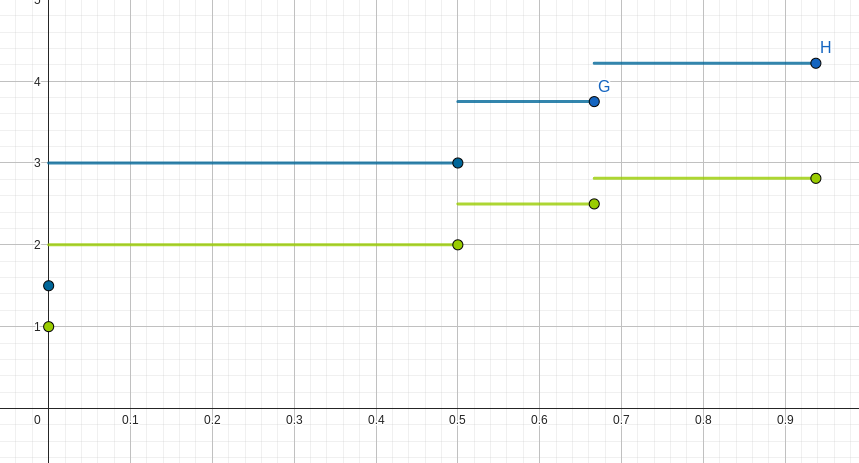
\includegraphics[width=1\linewidth]{fig2}
 	
 	
 	
 	
% \end{example} 




 \subsection{Operador de Poincaré} 
Si llamamos $\varphi_\alpha$  solución  del problema de valores iniciales
 \begin{equation}
 	\left\lbrace \begin{array}{l}
 		d\varphi=f(t,\varphi(t))d\mu\\
 		\varphi(0)=\alpha.
 	\end{array}\right. \label{eq:Problema 0}
 \end{equation}

A lo largo de la sección vamos a suponer que $ \mu$ es una medida de Borel positiva y finita, $f:[0,T]\times\rr^n\to\rr^n$ esta acotada, es decir $||f||_\infty<M$ y cumple con:
 \begin{enumerate}[label=\upshape(P-\arabic*),ref= (P-\arabic*)]
 	\item \label{pm1} Para cada $x\in\rr^n$, $f(t,x)$  $\mu$-medible en la variable $t$ y continua.
 	\item \label{pm2} Para cada $t\in[0,T]$, $f(t,x)$ es continua y acotada en la variable $x$, .
 	\item \label{pm3} Existen $a,b$ positivos tal que
 	$$|f(t,x)|\leq a|x|+b$$ 
 	\item \label{pm4}Existe $L\in\rr$ tal que $$\left| f(t,x)-f(t,y)\right|\leq L\left| x-y \right| . $$
 \end{enumerate} 
 Por el Teorema \ref{P-L}, para cada $\alpha$ existe una solución $\varphi_\alpha$ del problema de valores iniciales \ref{eq:Problema 0}. Veamos que propiedades tiene esta solución.
\begin{prop}
    $\varphi_{\alpha}\in L^\infty([0,T],\rr^n)$ y si $s\leq t$ entonces
    \begin{equation}\label{acotación}
        \left| \varphi_\alpha(t)-\varphi_\alpha(s)\right|\leq M\mu([s,t]).
    \end{equation}
\end{prop}
\begin{proof}[Dem:]
 	Si $\varphi_{\alpha}$ es solución del problema \ref{eq:Problema 0}, entonces por la ecuación (cita)

 		$$\varphi_{\alpha}(t)=\varphi_{\alpha}(0)+\int_{[0,t)} f(s,\varphi_{\alpha}(s))\;d\mu$$
$$ 		|\varphi_{\alpha}(t)| \leq |\varphi_{\alpha}(0)|+\int_{[0,t)}| f(s,\varphi_{\alpha}(s))|\;d\mu$$
luego por \ref{pm3}

\begin{equation*}
\begin{split}
 	|\varphi_{\alpha}(t)| \leq & |\varphi_{\alpha}(0)|+\int_{[0,t)}\left(a|\varphi_{\alpha}(s))|+b\right)\;d\mu\\	
     &\leq |\varphi_{\alpha}(0)|+b\mu([0,T])+a\int_{[0,t)}| \varphi_{\alpha}(s)|\;d\mu
\end{split}
\end{equation*}

 Si llamamos $C=|\varphi_{\alpha}(0)|+b\mu([0,T])$ y $\nu=a\mu$ entonces
 $$|\varphi_{\alpha}(t)| \leq C+\int_{[0,t)}| \varphi_{\alpha}(s)|\;d\nu$$
 aplicando el teorema \ref{TG} tenemos que pata $t\in[0,T]$
 \begin{equation*}
 	|\varphi_{\alpha}(t)|\leq CK(T)\exp\left(K(T)a\bar{\mu}([0,T]) \right)  < \infty
 \end{equation*}
Tomando supremo sobre todo el intervalo $[0,T]$, tenemos que\\ 
$\varphi_{\alpha}\in L^\infty([0,T],\rr^n).$
Por otro lado como $||f||_\infty \leq M$, para $s\leq t$
  	\begin{equation*}
  		|\varphi_\alpha(t)-\varphi_\alpha(s)|\leq \int_{[s,t)}|f(r,\varphi_\alpha(r))|\;d\mu\leq M\;\mu\left( [s,t) \right) 
  	\end{equation*}
\end{proof}
\begin{cor}\label{corolario_continuidad}
    Sea $\varphi_\alpha$ solución de \ref{eq:Problema 0}, entonces sea $t_0\in [0,T]$, si $\mu(\{t_0\})=0$ entonces $\varphi_\alpha$ es continua en $t_0$.
    
\end{cor}
\begin{proof}[Dem.]
Como $$0=\mu\left(\{t_0\}\right)=\mu\left(\bigcup_{n=1}^{\infty}\left[t_0-\frac{1}{n},t_0+\frac{1}{n}\right]\right)=\lim_{n\to\infty}\mu\left(\left[t_0-\frac{1}{n},t_0+\frac{1}{n}\right]\right)$$    
Para todo $\epsilon>0$ existe $N\in\nn$ tal que si $n>N$ entonces $$\mu\left(\left[t_0-\frac{1}{n},t_0+\frac{1}{n}\right]\right)<\epsilon/M.$$
Por la proposición \eqref{acotación}, existe $\delta>0$ tal que si $$t\in\left[t_0-\delta,t_0+\delta\right]\subset\left[t_0-\frac{1}{n},t_0+\frac{1}{n}\right]$$ entonces
\begin{equation}
    |\varphi_\alpha(t)-\varphi_\alpha(t_0)|\leq M\mu\left(\left[t_0-\frac{1}{n},t_0+\frac{1}{n}\right]\right)<\epsilon
\end{equation}
\end{proof}




El siguiente teorema muestras que las soluciones están definidas en todo $[0,T]$.

 
 \begin{thm}[\textbf{Dominio de la solución}]\label{th:P(T)}
 	Sea $\mu$ una medida de Borel finita , $f:[0,T]\times \rr^n\to\rr^n$ que cumple con las condiciones \ref{pm1}  a \ref{pm4},  entonces la solución del problema \ref{eq:Problema 0} esta definida en todo el intervalo $[0,T]$.
 \end{thm}
 \begin{proof}[Dem.]
 	Supongamos que la solución máxima esta definida en el intervalo $[0,t_1]$, donde $t_1< T$. Entonces por el Teorema  \ref{th:extensión} se debe cumplir alguna de las dos condiciones:
 	\begin{enumerate}
 		\item[A)] 	$\forall K\Subset [0,T)\times\rr^n$ existe $t_2\in [0,t_1)$ tal que $(t,\varphi(t))\notin K$   $\forall t\in(t_2,t_1)$. 

        \item[B)] Existe $x_1=\lim\limits_{t\to t_1^-}\varphi(t)$,  $(t_1,x_1)\in[0,T)\times\rr^n$ y  $$\left( t_1 , \varphi(t_1)+f(t_1,\varphi(t_1))\mu(\{t_1\})\right) \notin [0,T)\times\rr^n$$
\end{enumerate}


   
 	Si la condición (A) es verdadera entonces para
 		$\epsilon\in\left( 0,\dfrac{T-t_1}{2}\right) $ defino el conjunto $K_{\epsilon}=[0,t_1+\epsilon]\times B(0,R)$ donde $||\varphi||_\infty\leq R$. Como $K_{\epsilon}$ es cerrado y acotado entonces, $K_{\epsilon}$ está compactamente incluido en $[0,T)\times\rr^n$, luego existe $t_2\in [0,t_1)$ tal que $(t,\varphi(t))\notin K_{\epsilon}$ para todo $t\in(t_2,t_1)$. Como $\varphi(t)\in B(0,R)$, la única manera de que  $(t,\varphi(t))\notin K_{\epsilon}$, es que  $t>t_1+\epsilon$ lo cual es un absurdo.
   
   Por otro lado, es inmediato que  (B) es falso porque implicaria que  $\varphi(t_1)+f(t_1,\varphi(t_1))\mu(\{t_1\})\in\rr^n$.
 	
 		

 Luego el intervalo donde esta definida $\varphi$ es $[0,T]$.
 \end{proof}


\begin{defi}
 Llamaremos operador de Poincaré  al operador $P:\rr^n\to \rr^n$ tal que para cada valor inicial $\alpha$,\index{operador de Poincaré} $P(\alpha)=\varphi_\alpha(T)$, \index[Simbolo]{$P$} donde $\varphi_\alpha$ es solución de \ref{eq:Problema 0}.
\end{defi}

 
 \begin{lem}
    El operador de Poincaré es continuo.\label{opr continuo}
\end{lem}
\begin{proof}[Dem.]
 Sean $\varphi_\alpha$ y $\varphi_\beta$ dos soluciones del problema \eqref{eq:Problema 0}. Entonces, como $f$ es Lipschitz 
 \begin{equation*}
 \begin{split}
 	| \varphi_\alpha(t)-\varphi_\beta(t)|&\leq |\alpha-\beta |+\int_{[0,t)} |f(r,\varphi_\alpha(r)) -f(t,\varphi_\beta(t))| \; d|\mu|\\
	&\leq |\alpha-\beta|+L\int_{[0,t)} |\varphi_\alpha(r) -\varphi_\beta(t)| \; d|\mu|.
 \end{split}
\end{equation*}
 Si aplicamos el teorema \ref{TG} tomando $u(t)=|\varphi_\alpha(t)-\varphi_\beta(t)|$, $c=|\alpha-\beta|$ y  $\nu=L|\mu|$, entonces  

\begin{equation*}
|\varphi_\alpha(t)-\varphi_\beta(t)|\leq K(t) |\alpha-\beta|e^{K(t)L\bar{|\mu|}([t_0,t))}.
\end{equation*}
Luego si evaluamos en $t=T$ y llamamos  $K=K(T)=\displaystyle\prod_{\tau\in D}\mu(\{\tau\})<\infty$.
 

\begin{equation*}
 		|P(\alpha)-P(\beta)|=|\varphi_{\alpha}(T)-\varphi_{\beta}(T)|_{1}\leq K |\alpha-\beta|_{1}e^{KL\bar{|\mu|}([0,T))}\to 0
 	\end{equation*}
 cuando $|\alpha-\beta|\to 0$.
\end{proof}
 
 
 

%\begin{obs} \label{ob: cont P}
 %	Por \ref{th:P(T)}  el operador de Poincaré está bien definido, ya que la solución se puede extender a todo el intervalo $[0,T]$. Además por \ref{opr continuo} el operador es continuo.
 %\end{obs} 
 
 

 \begin{thm} \label{th: P}
 	Sea $R>0$ y $\varphi$ una solución del problema \ref{eq:Problema 0}, donde $f$ satisface las condiciones \ref{pm1} a \ref{pm4}, \ref{fun-tele} para $B(0,R)$  y  además que
 	\begin{equation}
 		f(t,u)\cdot u<0 \text{ para todo par } (t,u) \text{ donde }  |u| =R  \text{ y   } \mu(\{t\})=0.  \label{eq:4}
 	\end{equation}
 Entonces $P\left(  \overline{B(0,R)}\right)  \subset \overline{B(0,R)}$.
 \end{thm}
 
 \begin{proof}[Dem.]
 	Sea $A=\{t\in [0,T] \mid \varphi_\alpha(s)\in \overline{B(0,R)}, \; \forall s\in [0,t]\}$, veamos que el conjunto $A$ es simultáneamente abierto y cerrado relativo al intervalo $[0,T]$, y  como $[0,T]$ es conexo entonces $A=[0,T]$.
 	
 	Veamos primero que es un conjunto cerrado respecto al $[0,T]$. Para ello sea   $t_n$  una sucesión de $A$ que converge a $t$, veamos que $t\in A$.  Si para algún $n$, $t_n\geq t$ entonces $\forall s \in [0,t]\subset [0,t_n] $ vale que $\varphi(s)\in\overline{B(0,R)}$,  por lo tanto en $t\in A$.  Si por el contrario $\forall n$ tenemos que $t_n < t$,  como $\varphi$ es continua a izquierda, entonces $\lim\limits_{n\to \infty}\varphi(t_n)=\varphi(t)$ y como cada $\varphi(t_n)\in \overline{B(0,R)}$ entonces $\varphi(t)\in \overline{B(0,R)}$es decir $t\in A$ Por lo tanto $A$ es cerrado.
 	 
  	Si $A$ es un conjunto abierto relativo al $[0,T]$, entonces $[0,T]\setminus A$ es cerrado, es decir para toda sucesión $\{t_n\}\subset [0,T]\setminus A$ si $t_n\to t$ entonces $t\in[0,T]\setminus A$. Por lo tanto si suponemos que  $A$ no es abierto relativo al intervalo $[0,T]$, entonces $\exists t_0\in A$ y $\{t_n\}\nsubset A$ tal que $t_n\to t_0$. Podemos asegurar que si $t> t_0$ entonces $t\notin A$, pues tomando la sucesión $t_n=t_0-\left(\frac{t_0-t}{n}\right)$ tengo que $t_n\to t$, por lo tanto $t_n\notin A$ para todo $n$.
   
   Veamos que como $t_0\in A$, entonces $\varphi(t_0)\in B(0,R)$ o  $\varphi(t_0)\in \partial B(0,R) $, y siempre existe $t> t_0$ tal que $t\in A$.%$|\varphi(t)|\in \overline{B(0,R)}$.% 
 		\begin{itemize}
   		\item Si $\varphi(t_0)\in B(0,R)$
     \end{itemize}
    Tomando $x_1=\varphi(t_0)$ como condición inicial en el problema \ref{eq:Problema 0}, por el teorema \ref{P-L}  existe $\delta>0$ tal que \eqref{eq:Problema 0} tiene solución en el intervalo $[t_0,t_0+\delta)$, luego existe un $t\in(t_0.t_0+\delta)$ tal que $|\varphi(t)|\leq||\varphi||_\infty\leq R$. Por lo tanto $t\in A$ y $t>t_0$.
    
    \begin{itemize}
        
    
    \item Si $\varphi(t_0)\in \partial B(0,R)$ y $\mu(\{t_0\})\neq 0$
    
    \end{itemize}
Por \eqref{fun-tele} $x_1=\varphi(t_0)+f(t,\varphi(t_0))\mu(\{t_0\})\in B(0,R)$, y tomando la medida $\hat{\mu}=\mu-\mu(\{t_0\})\delta_{t_0}$, es claro que $\hat{\mu}(\{t_0\})=0$, puedo aplicar el teorema \ref{P-L} para la condición inicial $\varphi(t_0)=x_1$, pero con la medida $\hat{\mu}$. Luego existe $\delta>0$ tal que la solución a este nuevo problema esta definida en el intervalo $[t_0,t_0+\delta)$, como esta nueva solución para la medida $\hat{\mu}$ y para la medida $\mu$ difieren sólo en $t_0$ entonces, para $t\in (t_0,t_0+\delta)$ son iguales. Por lo tanto existe $t>t_0$ tal que $t\in A$.
% \begin{multline*}
 %	|\hat{\mu}|\left( \{t_0\}\right) =|\hat{\mu}|\left( \bigcap_{n=1}^\infty[t_0,t_0+1/n)\right)=\lim\limits_{n\to\infty}|\hat{\mu}|\left( [t_0,t_0+1/n) \right) =0
 %\end{multline*} 
 %existe $N>0$ que $|\hat{\mu}\left( [t_0,t_0+1/N]\right)\leq R/M $. Por lo tanto puedo aplicar el Teorema de Existencia y Unicidad para las condiciones $(t_0,x_1)$ y la medida $\hat{\mu}$, por el cual va a  existir $\delta$ tal que el problema \refeq{Problema P} tiene solución en el intervalo $[t_0,t_0+\delta]$,  es decir podemos extender la solución del problema hasta el intervalo $[0,t_0+\delta]$ lo cual contradice que $A$ no sea abierto.
 		



    
\begin{itemize}
\item Si $\varphi(t_0)\in \partial B(0,R)$ y $\mu(\{t_0\})= 0$ 
\end{itemize}
De \ref{eq:4} existe $b>0$ tal que $f(t_0,\varphi(t_0))\cdot\varphi(t_0)<-b$.

Por \ref{f lipschitz} y \ref{corolario_continuidad} para $\epsilon=\frac{b}{3RL}$ existe $\delta_1>0$ tal que si $t\in[t_0,t_0+\delta_1)$ entonces
\begin{equation}
    \begin{split}
        \int_{[t_0,t)} f(s,\varphi_\alpha(s))-f(s,\varphi_\alpha(t_0))\; d\mu& \leq \int_{[t_0,t)} |\varphi_\alpha(s)\varphi_\alpha(t_0)|\; d\mu \\ &\leq \frac{b}{3R}\mu((t_0,t))
    \end{split}\label{eq:A}
\end{equation}
Además como $f$ es continua en $t_0$ $\exists \delta_2>0 $ tal que si $s\in [t_0,t_0+\delta_2)$ entonces
\begin{equation}
    |f(s,\varphi_\alpha(t_0))-f(t_0,\varphi_\alpha(t_0))|\leq \frac{b}{3R}\label{eq:B}
\end{equation}

Para todo $t\in[t_0,t_0+\delta)$, donde $\delta=\min\{\delta_1,\delta_2\}$, usando \eqref{eq:A} y \eqref{eq:B} tenemos que 
\begin{equation*}
    \begin{split}
    \varphi_\alpha(t)-\varphi_\alpha(t_0) =& \int_{(t_0,t)}\left[f(s,\varphi_\alpha(s))-f(s,\varphi_\alpha(t_0))\right]\; d\mu\\& + \int_{(t_0,t)}\left[f(s,\varphi_\alpha(t_0))-f(t_0,\varphi_\alpha(t_0))\right]\; d\mu \\&+ \int_{(t_0,t)}f(t_0,\varphi_\alpha(t_0))\; d\mu,
    \end{split}
\end{equation*}
 \begin{equation*}
\begin{split}
\varphi_\alpha(t)-\varphi_\alpha(t_0) \leq \frac{b}{3R}\mu((t_0,t)) + \int_{(t_0,t)}\frac{b}{3R}\; d\mu + \int_{(t_0,t)}f(t_0,\varphi_\alpha(t_0))\; d\mu.
\end{split}
\end{equation*}		 
Si multiplico por el vector $\varphi_\alpha(t_0)$ y como $|\varphi_\alpha(t_0)|=R$, entonces
\begin{equation*}
\begin{split}
\left[\varphi_\alpha(t)-\varphi_\alpha(t_0)\right]\cdot \varphi_\alpha(t_0) \leq& \varphi_\alpha(t_0)\frac{2b}{3R}\mu((t_0,t)) + \int_{(t_0,t)}f(t_0,\varphi_\alpha(t_0))\cdot \varphi_\alpha(t_0)\; d\mu\\
&\leq \frac{2b}{3}\mu((t_0,t))-b\mu((t_0,t))=-\frac{b}{3}\mu((t_0,t)).
\end{split}
\end{equation*}
Luego por \eqref{acotación}
\begin{equation*}
    \begin{split}
    |\varphi_\alpha(t)|^2=&|\varphi_\alpha(t_0)|^2+2\left[\varphi_\alpha(t)-\varphi_\alpha(t_0)\right]\cdot\varphi_\alpha(t_0)+|\varphi_\alpha(t)-\varphi_\alpha(t_0)|^2\\
   &\leq R^2-\dfrac{2b}{3}\mu((t_0,t))+M^2 \mu((t_0,t))^2 ,  
    \end{split}
\end{equation*}
O equivalentemente
\begin{equation}
    |\varphi_\alpha(t)|^2-R^2\leq \mu((t_0,t))\left[M^2 \mu((t_0,t))-\dfrac{2b}{3}\right] 
\end{equation}
El termino de la derecha en es una expresión cuadrática respecto a $\mu((t_0,t))$, y tiene como raíces $t_0$ y otra a derecha de $t_0$, es decir existe $t_1>t_0$ tal que $|\varphi_\alpha(t_1)|^2-R^2\leq 0$, por lo tanto $t_1\in A$.
  		
 Por lo tanto mostramos que existe $t_1>t_0$ tal que $t\in A$, lo cual contradice que no sea abierto relativo al $[0,T]$. Entonces si $A$ es abierto y cerrado relativo al intervalo $[0,T]$, entonces $A=[0,T]$.
 	
Luego para cualquier $\alpha\in\overline{B(0,R)}$, $$P(\alpha)=\varphi_\alpha(T)\in\overline{B(0,R)}$$ 
 \end{proof}
 
 \begin{thm}[Teorema de Brouwer ]
 	
 	Sea $B(0,R)$ una bola de $\rr^n$  y sea $P:\overline{B(0,R)}\to \overline{B(0,R)}$ continua. Entonces existe $x \in \overline{B(0,R)}$ tal que $P(x) = x$.
 \end{thm}
 \begin{thm} \label{th:final}
 	Sea $\mu$ una medida de Borel finita, y sea $f:[0,T]\times\rr^n\to\rr^n$ una función que cumple con las condiciones \ref{pm1} a \ref{pm4}. Ademas existe una bola $B(0,R)$ tal que si $x\in\overline{B(0,R)}$ entonces $x+f(t,x)\mu(\{t\})\in \overline{B(0,R)}$ para todo $t\in[0,T]$, y
 	$$f(t,x)\cdot x<0 \; \text{ para todos}\; |x|=R \;\text{y}\; \mu(\{t\})=0.$$
 	Entonces el problemas
 	 \begin{equation}
 		\left\lbrace \begin{array}{l}
 			d(\varphi)=f(t,\varphi(t))d\mu\\
 			\varphi(0)=\varphi(T)
 		\end{array}\right. \tag{${PP}$}
 	\end{equation} 
tiene al menos una solución. 
\end{thm}
 \begin{proof}[Dem.]
 	Por el teorema \ref{th:P(T)} y el lema  \ref{opr continuo} el operador $P$ esta bien definido y es continuo. Luego por el Teorema \ref{th: P} $P\left( \overline{B(0,R)}\right)\subset\overline{B(0,R)} $, aplicando el teorema de Brouwer existe una solución $\varphi$ al problema \ref{eq:Problema 0} tal que $\varphi(T)=\varphi(0).$
 \end{proof}

 \begin{example}
 	Supongamos $u:[0,T]\to \rr$ que tenemos el siguiente problema
 	 \begin{equation*}
 		\left\lbrace \begin{array}{l}
 			d(u')=-g(u')- u+f(t,u,u')d\delta_{t_1}\\
 			u'(0)=u'(T)\\
 			u(0)=u(T)
 		\end{array}\right. 
 	\end{equation*} 
 donde $t_1\in(0,T)$, $g:\rr\to\rr$, $f:[0,T]\times\rr^2\to\rr$ y $d\delta_{t_1}$ la medida delta de dirac concentrada en $t_1$. Si llamamos $\lambda$ a la medida de Lebesgue entonces podemos escribir el problema de la siguiente manera
 \begin{equation*}
 	\left\lbrace \begin{array}{l}
 		d(u')=\left[ -g(u')- u\right] \chi_{[0,T]-\{t_1\}} +f(t,u,u')\chi_{\{t_1\}}d(\lambda+\delta_{t_1})\\
 		u'(0)=u'(T)\\
 		u(0)=u(T)
 	\end{array}\right. 
 \end{equation*} 
 Si llamamos $u'=v$ entonces tenemos el siguiente sistema
  \begin{equation*}
 	\left\lbrace \begin{array}{l}
 		u'=v\chi_{[0,T]-\{t_1\}}d(\lambda+\delta_{t_1})\\
 		d(v)=\left[ -g(v)- u \right] \chi_{[0,T]-\{t_1\}} +f(t,u,v)\chi_{\{t_1\}}d(\lambda+\delta_{t_1})
 	\end{array}\right. 
 \end{equation*} 
Si llamamos $\varphi(t)=(u(t),v(t))$ entonces suponiendo que $v(0)=v(T)$ tenemos que
  \begin{equation*}
	\left\lbrace \begin{array}{l}
		d(\varphi)=\left( v\chi_{[0,T]-\{t_1\}},\left[ -g(v)- u\right] \chi_{[0,T]-\{t_1\}} +f(t,u,v)\chi_{\{t_1\}}\right) d(\lambda+\delta_{t_1})\\
		\varphi(0)=\varphi(T)
	\end{array}\right. 
\end{equation*} 
si llamamos $F(t,\varphi)=\left( v\chi_{[0,T]-\{t_1\}}, \left[ -g(v)-u\right] \chi_{[0,T]-\{t_1\}} +f(t,u,v)\chi_{\{t_1\}}\right) $ y $d\mu=d(\lambda+\delta_{t_1})$. Por el teorema \ref{th:final} va a existir una solución si 
\begin{itemize}
	\item Siempre que $|(u,v)|=R$ entonces si $(\lambda+\delta_{t_1})(\{t\})=0$ 
	$$\left(v\chi_{[0,T]-\{t_1\}}, \left[ -g(v)- u\right] \chi_{[0,T]-\{t_1\}} +f(t,u,v)\chi_{\{t_1\}}\right) \cdot (u,v)<0.$$
	
	Como $(\lambda+\delta_{t_1})(\{t\})=0$ solo cuando $t\neq t_1$ solo nos hace falta que 
	$$vu-g(v)v- uv <0$$ 
	$$g(v)v>0$$
	lo cual vale si pedimos que $g(v)<0$ si $v<0$ y $g(v)>0$ si $v>0$.
	
	
	\item Si $(u,v)\in\overline{ B(0,R)}$ entonces
	$$(u,v)+\left(v\chi_{[0,T]-\{t_1\}}, \left[ -g(v)-u\right] \chi_{[0,T]-\{t_1\}} +f(t,u,v)\chi_{\{t_1\}}\right) (\lambda+\delta_{t_1})(\{t\})\in \overline{ B(0,R)}$$
	El único caso en el que podría no pasar es cuando $(\lambda+\delta_{t_1})(\{t\})\neq 0$ po lo cual necesitamos que
	$$\left\| (u,v)+(0,f(t_1,u,v))\right\|^2\leq R^2 $$
		$$\left\| (u,v+f(t_1,u,v))\right\|^2\leq R^2 $$
	o lo que es lo mismo	$u^2+v^2+2vf(t_1,u,v)+(f(t_1,u,v))^2\leq R^2$, y como $u^2+v^2\leq R^2$ entonces
	$$2vf(t,u,v)+(f(t_1,u,v))^2\leq 0$$
	lo cual es una parábola cuyas raíces son $0$ y $-2v$, es decir solo necesitamos que $f(t_1,u,v)\in B(0,2|v|)$.
\end{itemize}
Luego el problema 
\begin{equation*}
	\left\lbrace \begin{array}{l}
		d(u')=-g(u')- u+f(t,u,u')d\delta_{t_1}\\
		u'(0)=u'(T)\\
		u(0)=u(T)
	\end{array}\right. 
\end{equation*} 
tendrá solución si para todo $(x,y)\in B(0,R)$ $g(v)<0$ si $v<0$ y $g(v)>0$ si $v>0$, y $|f(t,x,y)|\leq 2|y|$. 
 \begin{itemize}
 	\item  Por ejemplo si tomamos $g(y)=y^3$ y $f(t,x,y)=ky$ donde $k<2$ entonces 
\begin{equation*}
	\left\lbrace \begin{array}{l}
		d(u')=-(u')^3- u+ku' d\delta_{t_1}\\
		u(0)=u(T)
	\end{array}\right. 
\end{equation*} 
tiene solución en $ \rr^2$.

\item  Si tomo $g(y)=\sen(y)$ y $f(t,x,y)=ky$  donde $k<2$ entonces
\begin{equation*}
	\left\lbrace \begin{array}{l}
		d(u')=-\sen(u')- u+ku' d\delta_{t_1}\\
		u(0)=u(T)
	\end{array}\right. 
\end{equation*} 
tiene solución en $ \rr\times [-\pi,\pi]$.
\item Si en la ecuación del péndulo forzado suponemos que para angulos chicos $u = sen(u)$ entonces la ecuación del péndulo forzado es 
\begin{equation*}
	\left\lbrace \begin{array}{l}
		d(u')=-u-u'+ku' d\delta_{t_1}\\
		u(0)=u(T)
	\end{array}\right. 
\end{equation*} 

\end{itemize}
 \end{example}
\chapter{Experimentos Númericos}
\section{Método Numérico }
 
\begin{example}
Vamos a tomar la siguiente ecuación diferencial 
\begin{equation}
	\left\lbrace \begin{array}{l}
		d(u')=-u' d\delta_{\hat{t}}\\
		u(0)=0\\
		u'(0)=1
	\end{array}\right. \label{eq:3.1}
\end{equation} 
Donde $d\delta_{\hat{t}}(A)=\left\lbrace \begin{array}{l}
	0 \; si \; \hat{t}\notin A\\
	1 \; si \; \hat{t}\in A
\end{array}\right. $

Una solución de \ref{eq:3.1}   es una función de variación acotada y continua a izquierda $u'$ tal que  para cualquier conjunto $A$ de Borel
\begin{equation*}
	\mu_{u'}(A)=\int_A-u'(s)\: d\delta_{\hat{t}}(s)
\end{equation*}
donde $\mu_{u'}$ es la medida generada por $u'$. Si tomamos el intervalo $[0,t)$ entonces 
$$u'(t)-u'(0)=\mu_{u'}([0,t))=\int_{[0,t)}-u'(s)\: d\delta_{\hat{t}}(s)$$
 Podemos trasformar esta ecuación \ref{eq:3.1} en un sistema de ecuaciones de la siguiente manera
 \begin{multicols}{2}

 	$\left\lbrace \begin{array}{l}
 		d(u)=vd\lambda\\
 		d(v)=-v d\delta_{\hat{t}}\\
 		u(0)=0\\
 		v(0)=1
 	\end{array}\right. $
 
 	$\left\lbrace \begin{array}{l}
 		u(t)=\displaystyle\int_{0}^{t}v(s) \; ds\\
 		\\
 		v(t)=1-\displaystyle\int_{[0,t)}v(s) \; d\delta_{\hat{t}}(s)
 	\end{array}\right. $
 
\end{multicols}
%cuya solución es
%
%
%\begin{multicols}{2}
%$v(t)=\left\lbrace \begin{array}{l}
%			1 \; si \; t\leq \hat{t}\\
%			0 \; si \; t> \hat{t}
%		\end{array}\right. $
%				 
%			$u(t)=\left\lbrace \begin{array}{l}
%				t \; si \; t\leq \hat{t}\\
%				\hat{t} \; si \; t> \hat{t}
%			\end{array}\right. $
%\end{multicols}
%
%
%


Si tomamos la partición del intervalo $[0,T]$, 
$$P_N=\{0=t_0,t_1, t_2,\cdots,t_n\cdots, t_N=T\}$$
podemos aproximar $$\displaystyle\int_{[0,t_n)}v(s) \; d\delta_{\hat{t}}(s) \approx \sum_{j=1}^{n-1}v(t_j)\delta_{\hat{t}}\left( [t_j,t_{j+1})\right), $$ donde $\{t_0=0,t_1,\cdots , t_n\}\subset P_N$. Entonces 
	\begin{equation*}
		v(t_n)=v(t_0)-\sum_{j=1}^{n-1}v(t_j)\delta_{\hat{t}}\left( [t_j,t_{j+1})\right) 
	\end{equation*}
si desarrollamos tenemos que
$$\begin{array}{l}
	v(t_1)=v(t_0)\\
	v(t_2)=v(t_0)-v(t_1)\delta_{\hat{t}}([t_1,t_2))=v(t_1)-v(t_1)\delta_{\hat{t}}([t_1,t_2))\\
	v(t_3)=v(t_0)-v(t_1)\delta_{\hat{t}}([t_1,t_2))-v(t_2)\delta_{\hat{t}}([t_2,t_3))=v(t_2)-v(t_2)\delta_{\hat{t}}([t_2,t_3))\\
	\cdots\\
	v(t_n)=v(t_{n-1})-v(t_{n-1})\delta_{\hat{t}}([t_{n-1},t_n))
\end{array}$$
Como vamos a poder encontrar un $1<r<N$ tal que $\hat{t}\in [t_r,t_{r+1})$. Entonces
\begin{itemize}
	\item  $v(t_i)=1$ para $i=1\cdots r$, pues $\delta_{\hat{t}}\left( [t_i,t_{i+1})\right)=0$
	\item$v(t_{r+1})=1-v(t_{r})\delta_{\hat{t}}\left( [t_{r},t_{r+1})\right)=1-\delta_{\hat{t}}\left( [t_{r},t_{r+1})\right)=0$
	\item $v(t_i)=0$ para $i=r+1, \cdots ,N$
\end{itemize}


Luego para la partición $P_N$ tenemos que
	 \begin{equation*}
		v(t_n)=\left\lbrace \begin{array}{l}
			1 \; si \; t_n\leq \hat{t}\\
			0 \; si \; t_n> \hat{t}
		\end{array}\right. 
	\end{equation*} 
Ya teniendo $v$ puedo resolver $u$ integrando con respecto a la integral de Lebesgue:
	 \begin{equation*}
	u(t_n)=\left\lbrace \begin{array}{l}
		t _n\; si \; t\leq \hat{t}\\
		\hat{t} \; si \; t_n> \hat{t}
	\end{array}\right. 
\end{equation*} 
Entonces si agrandamos la partición del intervalo $[0,T]$ tenemos 
\begin{center}
		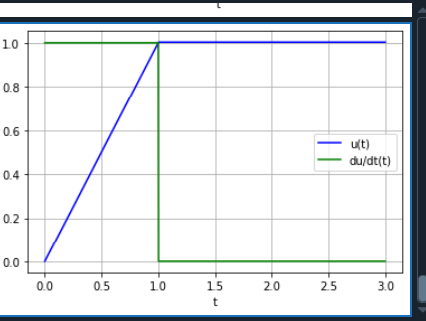
\includegraphics[width=0.7\linewidth]{fig3}
\end{center}
\vspace{0.2cm}
	
 Si aproximamos $\displaystyle\int_{[0,t_n)}v(s) \; d\delta_{\hat{t}}(s) \approx \sum_{j=1}^{n-1}\left( \dfrac{v(t_{j+1})+v(t_j)}{2}\right) \delta_{\hat{t}}\left( [t_j,t_{j+1})\right) $, donde $\{0=t_0,t_1,\cdots , t_n\}\subset P_N$. Entonces 
\begin{equation*}
	v(t_n)=v(t_0)-\sum_{j=1}^{n-1}\left( \dfrac{v(t_{j+1})+v(t_j)}{2}\right) \delta_{\hat{t}}\left( [t_j,t_{j+1})\right)
\end{equation*}
si desarrollamos tenemos que
$$\begin{array}{l}
	v(t_1)=v(t_0)\\
	v(t_2)=v(t_0)-\left[ \dfrac{v(2)+v(1)}{2}\right] \delta_{\hat{t}}([t_1,t_2))=v(t_1)-\left[ \dfrac{v(2)+v(1)}{2}\right] \delta_{\hat{t}}([t_1,t_2))\\
	v(t_3)=v(t_0)-\left[ \dfrac{v(2)+v(1)}{2}\right]\delta_{\hat{t}}([t_1,t_2))-\left[ \dfrac{v(3)+v(2)}{2}\right]\delta_{\hat{t}}([t_2,t_3))\\
	v(t_3)=v(t_2)-\left[ \dfrac{v(3)+v(2)}{2}\right]\delta_{\hat{t}}([t_2,t_3))\\
	\cdots\\
	v(t_n)=v(t_{n-1})-\left[ \dfrac{v(n)+v(n-1)}{2}\right] \delta_{\hat{t}}([t_{n-1},t_{n}))
\end{array}$$

Como vamos a poder encontrar un $1<r<N$ tal que $\hat{t}\in [t_r,t_{r+1})$. Entonces
\begin{itemize}
	\item  $v(t_i)=1$ para $i=1\cdots r$, pues $\delta_{\hat{t}}\left( [t_i,t_{i+1})\right)=0$
	\item $v(t_{r+1})=1-\dfrac{v(t_{r+1})}{2}$ luego $v(t_{r+1})=3/2$
	
	\item$v(t_{r+2})=3/2-\left[ \dfrac{v(r+2)+3/2}{2}\right]\delta_{\hat{t}}\left( [t_{r+1},t_{r+2})\right)=3/2$
	\item $v(t_i)=3/2$ para $i=r+1, \cdots ,N$
\end{itemize}
Entonces


\begin{equation*}
	v(t_n)=\left\lbrace \begin{array}{lcr}
		1 & si & t_n\leq \hat{t}\\
		2/3 & si & t_n> \hat{t}
	\end{array}\right. 
\end{equation*} 
Ya teniendo $v$ puedo resolver $u$ integrando con respecto a la integral de Lebesgue:
\begin{equation*}
	u(t_n)=\left\lbrace \begin{array}{lcr}
		t_n & si & t_n\leq \hat{t}\\
		\dfrac{2t_n+\hat{t}}{3} & si & t_n> \hat{t}
	\end{array}\right. 
\end{equation*} 
Entonces si agrandamos la partición del intervalo $[0,T]$ tenemos 
\begin{center}
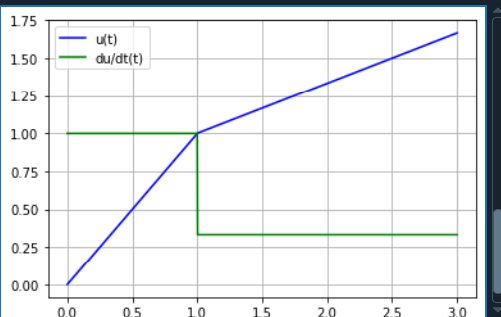
\includegraphics[width=0.7\linewidth]{fig4}
\end{center}
\end{example}
 
 
 \subsubsection{Método de Euler}
 Partimos del problema
 \begin{equation}
 	\left\lbrace \begin{array}{l} 
 			d(v)=f(t,v) d\mu\\
 			v(0)=v_0
 			\end{array}\right. \label{eq:3.2}
 \end{equation} 
 donde $f$ es una función Lipschitz en la variable vectorial, ademas $||f(t,v)||\leq \beta(t)\alpha(v)$. Una solución del problema \ref{eq:3.2} es una función continua izquierda y de variación acotada $v$ tal que
 \begin{equation}
 	v(t)=v(0)+\int_{[0,t)}f(s,v(s))\: d\mu(s) \label{eq:3.3}
 \end{equation}
 
 Queremos encontrar un algoritmo numérico para llar la solución de \ref{eq:3.2}, para ello necesitamos particionar el intervalo $[0,T]$, en $n+1$ puntos igualmente espaciados. Tenemos la partición $P_N=\{0=t_0,\cdots,t_N=T\}$  y partimos de suponer que 
 $$\int_{[t_i,t_{i+1})}f(s,v(s))\:d\mu(s)\approx f(t_i,v(t_i))\mu([t_i,t_{i+1}))$$
 
 Si llamamos $v_{i}$ a la aproximación de $v(t_i)$ mediante la suposición anterior  y  \ref{eq:3.3}, entonces 
 

 $$v_{i}=v_{i-1}+f(t_{i-1})\mu([t_{i-1},t_{i}))$$

\begin{obs}
	Sea $\mu$ es una medida de Borel, continua y finita. Si $\mu([0,T])<\infty$ entonces para la partición $P_N$ tenemos que $\exists R>0$ tal que $$\mu([t_{i-1},t_1))\leq \dfrac{R}{N}$$
\end{obs}
\begin{obs}
	Sea $v$ una función de variación acotada, entonces para la partición $P_N$  $\exists V>0$ tal que
	$$\V(v,[t_{i-1},t_i))\leq \dfrac{V}{N}$$ 
\end{obs}
\textbf{Veamos que error cometemos con este método.}
Si dividimos la medida $\mu$ en suma de una medida continua $\bar{\mu}$ y una discontinua $\mu_a$ según la definición \ref{mu_a}.
\begin{itemize}
	\item  Si consideramos la ecuación \ref{eq:3.2} donde $\mu$ es una medida continua entonces el error del método de Euler es el siguiente:


 Partiendo de que $v(0)=v_0$, para el valor $t_1$ se comete el siguiente error :
\begin{multline*}
	|v(t_1)-v_1|=\left| v(0)+\int_{[0,t_1)}f(s,v(s))\; d\mu(s)-v(0)-f(0,v(0))\mu([0,t_1))\right| \\
	\leq \int_{[0,t_1)}|f(s,v(s))-f(0,v(0))|\; d\mu(s)\leq L\int_{[0,t_1)}|v(s)-v(0)|\; d\mu(s)\\
	\leq L \V(v,[0,t_1))\mu([0,t_1))
\end{multline*}
 Por las observaciones  tenemos que 
 \begin{equation}
 	|v(t_1)-v_1|\leq L \V(v,[0,t_1))\mu([0,t_1))\leq L\dfrac{VR}{N^2}
 \end{equation}
 Para $t_2$ el error sera
\begin{multline*}
	|v(t_2)-v_2|=\left| v(0)+\int_{[0,t_2)}f(s,v(s))\; d\mu(s)-v_1-f(t_1,v_1)\mu([t_1,t_2))\right| \\
	=\left| v(0)+\int_{[0,t_1)}f(s,v(s))\; d\mu(s)+\int_{[t_1,t_2)}f(s,v(s))\; d\mu(s)-v_1-f(t_1,v_1)\mu([t_1,t_2))\right| 
\end{multline*}

\begin{multline*}
	|v(t_2)-v_2|	\leq |v(t_1)-v_1|+\left|\int_{[t_1,t_2)}f(s,v(s))\; d\mu(s)-f(t_1,v_1)\mu([t_1,t_2))\right| \\
	\leq |v(t_1)-v_1|+L \int_{[t_1,t_2)}|v(s)-v_1|\; d\mu(s)\\
		\leq |v(t_1)-v_1|+L \int_{[t_1,t_2)}|v(s)-v(t_1)+v(t_1)-v_1|\; d\mu(s)\\
			\leq |v(t_1)-v_1|+L \int_{[t_1,t_2)}|v(s)-v(t_1)|\; d\mu(s)+L\int_{[t_1,t_2)}|v(t_1)-v_1|\; d\mu(s)\\
			\leq |v(t_1)-v_1|+L \int_{[t_1,t_2)}|v(s)-v(t_1)|\; d\mu(s)+L|v(t_1)-v_1|\mu([t_1,t_2))\\
			\leq (1+L\dfrac{R}{N})|v(t_1)-v_1|+\int_{[t_1,t_2)}|v(s)-v(t_1)|\; d\mu(s)\\
	\leq (1+L\dfrac{R}{N})|v(t_1)-v_1|+L\dfrac{VR}{N^2}
\end{multline*}
 Por lo tanto podemos concluir que el error en el paso $i$-ésimo es 
\begin{equation}
		|v(t_{i})-v_i|\leq(1+L\dfrac{R}{N})|v(t_{i-1})-v_{i-1}|+L\dfrac{VR}{N^2}
\end{equation}
si reemplazo el error de las aproximaciones anteriores tengo

\begin{multline*}
	|v(t_{i})-v_i|\leq\left( 1+L\dfrac{R}{N}\right) ^{i-1}|v(t_{0})-v_{0}|+\left[ 1+\left( 1+\dfrac{R}{N}\right) +\cdots+\left( 1+\dfrac{R}{N}\right) ^{i-1}\right] \dfrac{LVR}{N^2}\\
	\leq\left( 1+L\dfrac{R}{N}\right) ^{i-1}|v(t_{0})-v_{0}|+\left[ \dfrac{1-\left( 1+\dfrac{R}{N}\right)^{i-1} }{1-\left(1+\dfrac{R}{N} \right) }\right] \dfrac{LVR}{N^2}\\
	\leq\left( 1+L\dfrac{R}{N}\right) ^{i-1}\left[ |v(t_{0})-v_{0}|+\dfrac{V}{N}\right] 
\end{multline*}
Si tenemos en cuenta que $|v(0)-v_0|=0$ y que $0\leq (1+x)^n\leq e^nx$ entonces
\begin{equation}
	|v(t_i)-v_i|\leq e^{-\frac{(i-1)R}{N}}\dfrac{V}{N}
\end{equation}
Por lo tanto el error global del método de Euler tiende a $0$ cuando $N$ tiende a infinito.


\item Si consideramos al problema \ref{eq:3.2} pero ahora para la medida $\mu_a$, definida en \ref{mu_a}.
\begin{obs}
	Si $\mu$ es una medida de Borel positiva y finita y $D=\{\tau\in [0,T]/ \mu(\{\tau\})>0\}$ vale que
	$$\mu_a([0,T])=\sum_{D}\mu(\{\tau\})\leq \mu([0,T])$$
	 Entonces para la partición $P_N$  existe $R=\displaystyle\max_{1\leq i\leq N}\{\mu_a([t_{i-1},t_i])\}$ tal que
	 $$\mu_a([t_{i-1},t_))\leq \dfrac{R}{N}$$
	 
	
	
\end{obs}





\end{itemize}
 
 
 
 
 
 
 
 
 
%%%%%%%%% medidas continuas %%%%%%%%
% 
% \begin{defi} 	Sea $\mu$ una medida de Borel.
% 	\begin{itemize}
% 		\item  Diremos que es regular si $\forall A\in\rr$ existe un conjunto de borel $B$ tal que $A\subset B$ y $\mu(A)=\mu(B)$.
% 		\item Diremos que es de Radom, si es regular y ademas para todo compacto $K$, $\mu(K)<\infty$.
% 	\end{itemize}
% \end{defi}
% 
%\begin{thm}
%	Sea $\mu$ y $\{\,u_k\}$  medidas de radom, entonces son equivalentes.
%	\begin{enumerate}
%		\item [i)] $\displaystyle\lim\limits_{k\to \infty}\int f\: d\mu_k=\int f d\:\mu$ para todo $f\in C_c(\rr)$.%% funciones continuas de soporte compacto
%		\item[ii)]$\limsup\limits_{k\to\infty}\mu_k(K)\leq \mu(K)$ para todo compacto $K\in\rr$ y $\mu(U)\leq \liminf\limits_{k\to\infty}\mu_k(U)$ para todo conjunto abierto $U\in\rr$.
%		\item [iii)]$\lim\limits_{k\to\infty} \mu_k(B)=\mu(B)$ para todo juntonto acotado de Borel con $\mu(\partial B)=0$.
%	\end{enumerate}
%\end{thm}
% \begin{proof}
% 	lo saque de \cite{Evanz}
% \end{proof}
% \begin{defi}
% 	Si se cumple alguna de las condiciones anteriores diremos que $\mu_k$ converge débil a $\mu$ y  lo notaremos
% 	$$\mu_{k}\rightharpoonup \mu$$
% \end{defi}
% 
% \begin{thm}[Convergencia Débil]
% 	Sea $\{u_k\}_{k=1}^\infty$ una sucesión de medidas de Radom que satisface que $\sup_k \{\mu(K)\}<\infty$ para todo compacto $K\subset [0,T]$, entonces existe una subsucesión $\mu_{k_n}$ y una medida de radom $\mu$ tal que  
% 	$$\mu_{k_n}\rightharpoonup \mu$$
% \end{thm}
% 
% 
% Sea $\mu_k$  una medida de radom,  tal que $$\mu_k(A)=\int_AH_k(t)dt$$
% donde $H_k$ es una función continua. Supongamos que $\mu_{k}\rightharpoonup \mu$.
% Sea $\varphi_k$ una solución del problema \ref{Problema P} con la medida continua $\mu_k$, entonces para todo conjunto de Borel $A$ $$\mu_{\varphi_k}(A)=\int_A f(t,\varphi_k(t)) \: d\mu_k(t)$$
% 
%Veamos que $\mu_{\varphi_k}\rightharpoonup \mu_\varphi$.
% 
% 
 
 







\printindex
\printindex[Simbolo]
\bibliographystyle{plain}
\bibliography{lib_tesis}
%\begin{thebibliography}{10}
	
	%\bibitem{Amster} \textsc{Pablo Amster}- Topological Methods in the Study of Boundary Value Problems, Springer 2014.
	
	%\bibitem{Evanz} \textsc{Lawrence Craig Evans}- Measure Theory and Fine Properties of Func 
	
	%\bibitem{P.Mazzone} \textsc{Gastón Beltritti, Stefania Demaria,
	%Graciela Giubergia, Fernando Mazzone }-The Picard-Lindelof theorem and continuation of solutions for measure diferential equations.
	
	%\bibitem{Evanz} \textsc{Evans, L.C. y Gariety, R.F.}-Measure Theoty and Finite properties of functions. 
	
	%\bibitem{Zo} \textsc{Norberto Fava y Felipe Zo}- Medida e Integral de Lebesgue, RED OLIMPICA 1996.
	
	%\bibitem{M-W} \textsc{Jean Mawhin Michel Willem} -Critical Point Theory and Hamiltonian Systems, Springer-Verlag
	
	%\bibitem{Carter}\textsc{M. Carter, B. vam Brunt}- The Lebesgue-
	%Stieltjes Integral: A Practical Introduction,
	%Springer Science \& Business Media, 2000. Zbl 0948.28001, DOI 10.1007/978-1-4612-1174-7.
	
	%\bibitem{limits}\textsc{D. Applebaum}- Limits, Limits Everywhere: The Tools of Mathematical Analusis.
	
	%\bibitem{folland}\textsc{Folland G.}, Real  Analysis: Modern techniques and their applications , (2ed., PAM, Wiley, 1999).
	
%\end{thebibliography}






\end{document}
